 
\section{Pre-Fit Plots}
\label{sec:app-controlPlots}


\subsection{$tWZ$ OF SR}
\label{sec:app-controlplotstetralepton-tWZ-OF-SR}

\begin{figure}[htbp]
  \centering
  \begin{tabular}{ccc}

    %%%%%%%%%%%%%%%
    %%% Leptons %%%
    %%%%%%%%%%%%%%%


    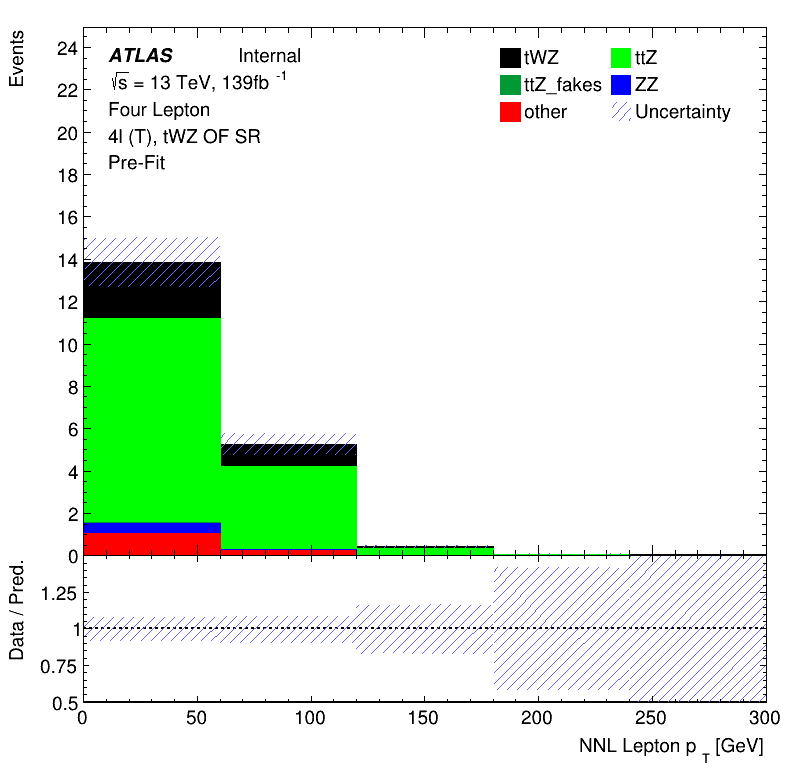
\includegraphics[width=.2\textwidth]{figures/PreFitPlots/lep4_tWZ_4T_OF_NNL_lepton_pt} &
    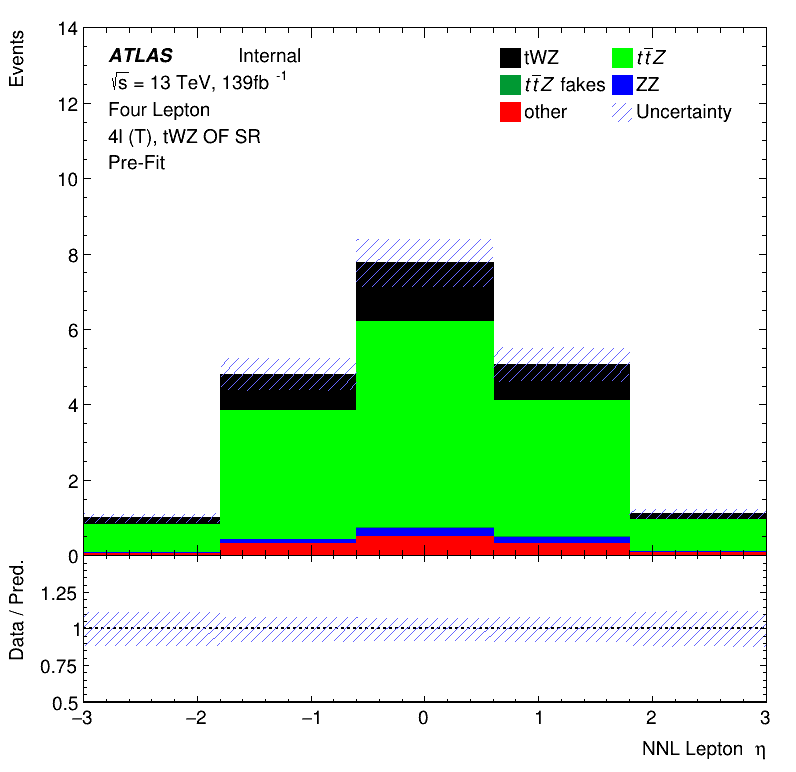
\includegraphics[width=.2\textwidth]{figures/PreFitPlots/lep4_tWZ_4T_OF_NNL_lepton_eta} &
    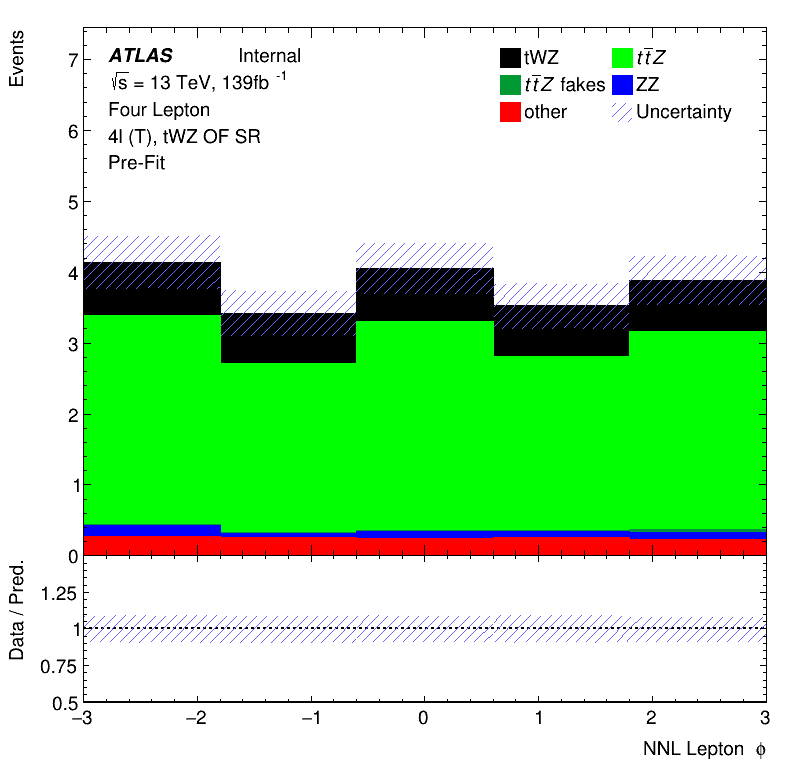
\includegraphics[width=.2\textwidth]{figures/PreFitPlots/lep4_tWZ_4T_OF_NNL_lepton_phi} \\
    \multicolumn{3}{c}{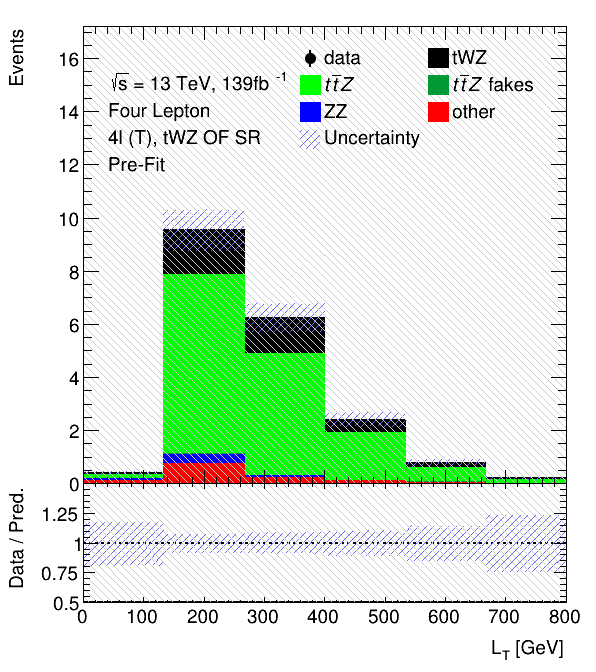
\includegraphics[width=.2\textwidth]{figures/PreFitPlots/lep4_tWZ_4T_OF_LT} }\\

  \end{tabular}
  \caption{Top row: MC predictions for $p_{T}$, $\eta$ and $\phi$ for next-to-next-to-leading (NNL) leptons in the $tWZ$ OF SR region (\textit{blinded}). Bottom row: MC predictions for $L_{T}$ (scalar sum of lepton $p_{T}$)  in the $tWZ$ OF SR region (\textit{blinded})}
  \label{fig:4lep-OF-SR-leptonPlots}
\end{figure}


\begin{figure}[htbp]
  \centering
  \begin{tabular}{ccc}
    %%%%%%%%%%%%%%%%%
    %%% electrons %%%
    %%%%%%%%%%%%%%%%%


    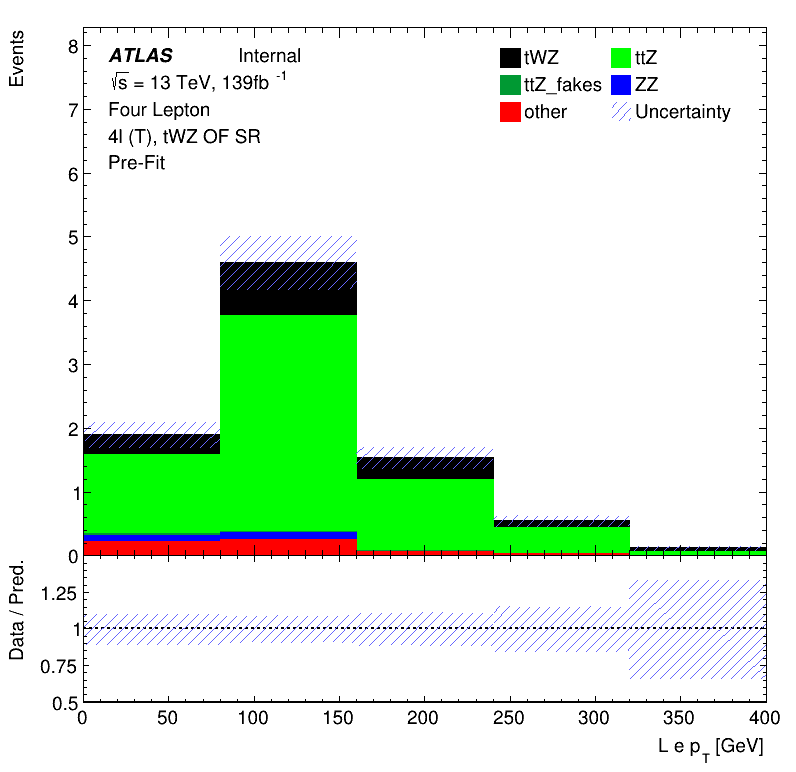
\includegraphics[width=.2\textwidth]{figures/PreFitPlots/lep4_tWZ_4T_OF_L_el_pt} &
    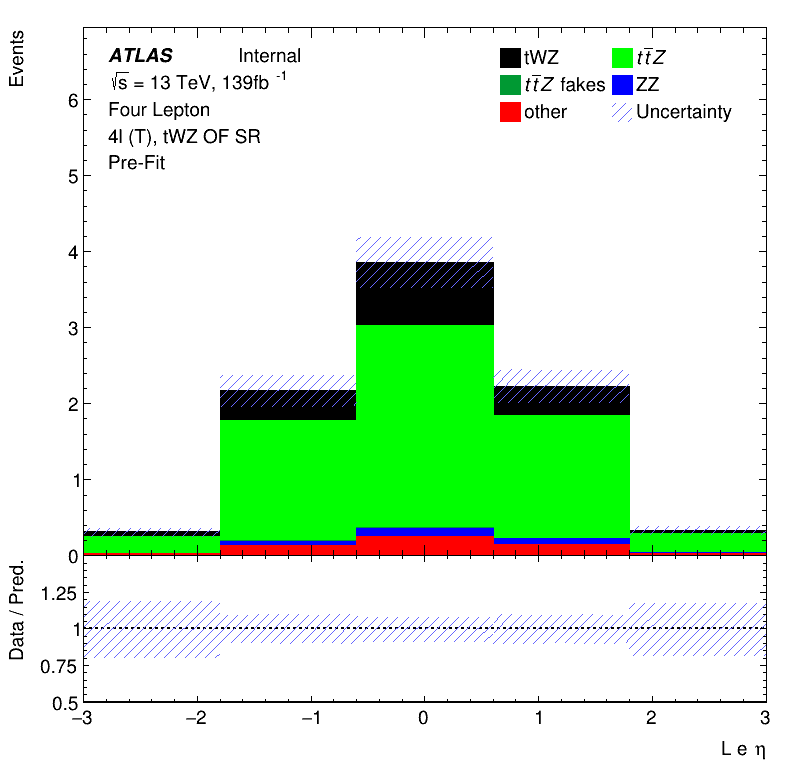
\includegraphics[width=.2\textwidth]{figures/PreFitPlots/lep4_tWZ_4T_OF_L_el_eta} &
    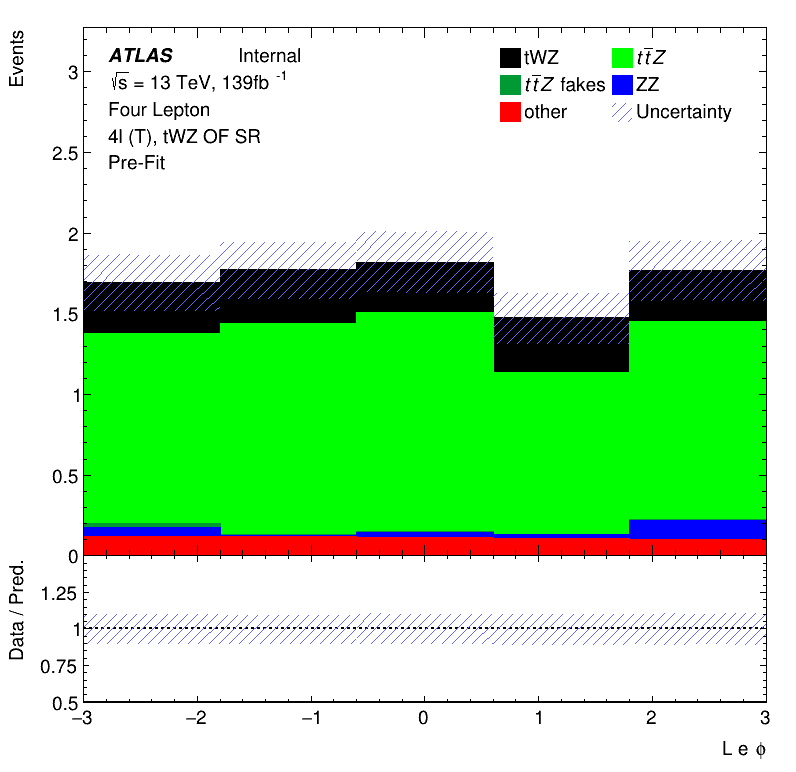
\includegraphics[width=.2\textwidth]{figures/PreFitPlots/lep4_tWZ_4T_OF_L_el_phi} \\
    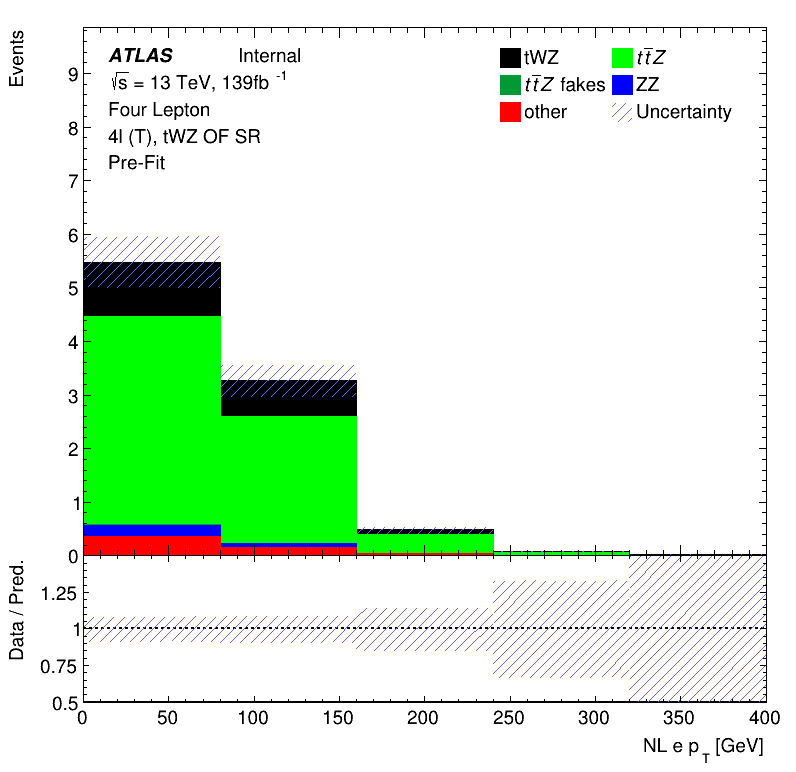
\includegraphics[width=.2\textwidth]{figures/PreFitPlots/lep4_tWZ_4T_OF_NL_el_pt} &
    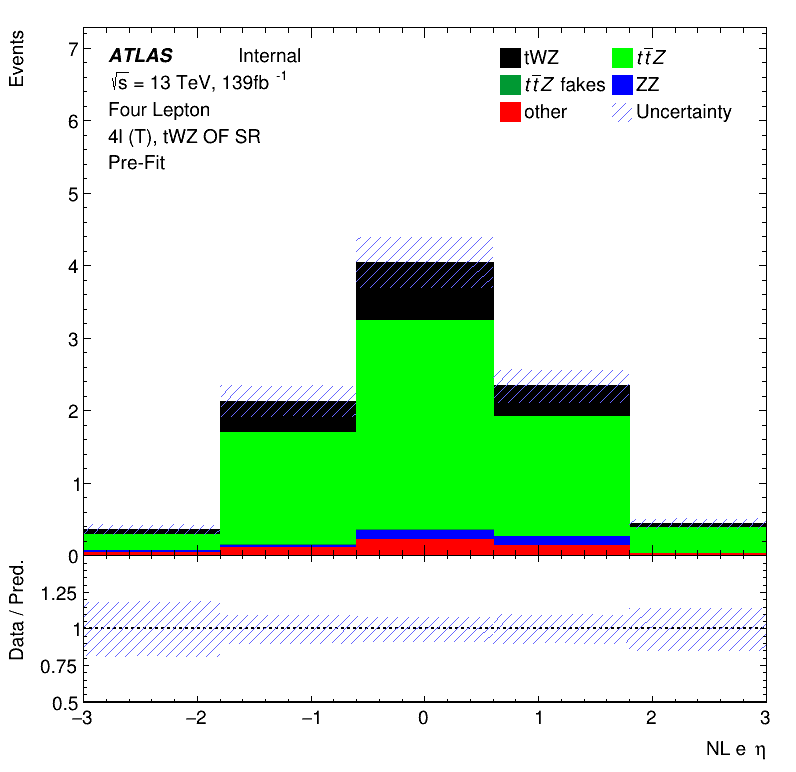
\includegraphics[width=.2\textwidth]{figures/PreFitPlots/lep4_tWZ_4T_OF_NL_el_eta} &
    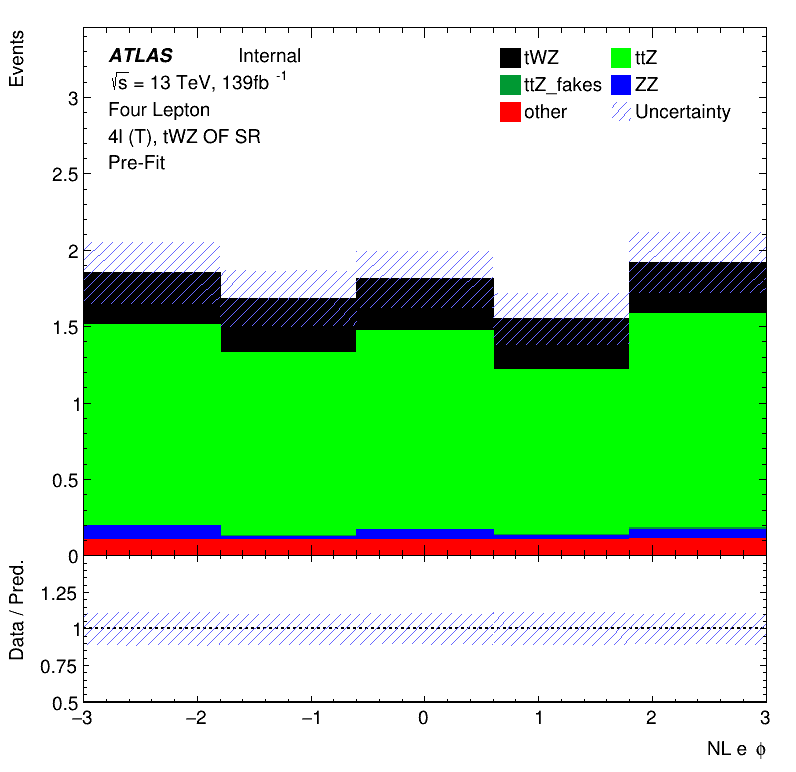
\includegraphics[width=.2\textwidth]{figures/PreFitPlots/lep4_tWZ_4T_OF_NL_el_phi} \\

  \end{tabular}
    \caption{MC predictions for $p_{T}$, $\eta$ and $\phi$ for leading (L) electrons (top row) and next-to-leading (NL) electrons (bottom row) in the $tWZ$ OF SR region (\textit{blinded})}
  \label{fig:4lep-OF-SR-electronPlots}
\end{figure}

\clearpage

\begin{figure}[htbp]
\centering
  \begin{tabular}{ccc}
    %%%%%%%%%%%%%%%%%
    %%% electrons %%%
    %%%%%%%%%%%%%%%%%

    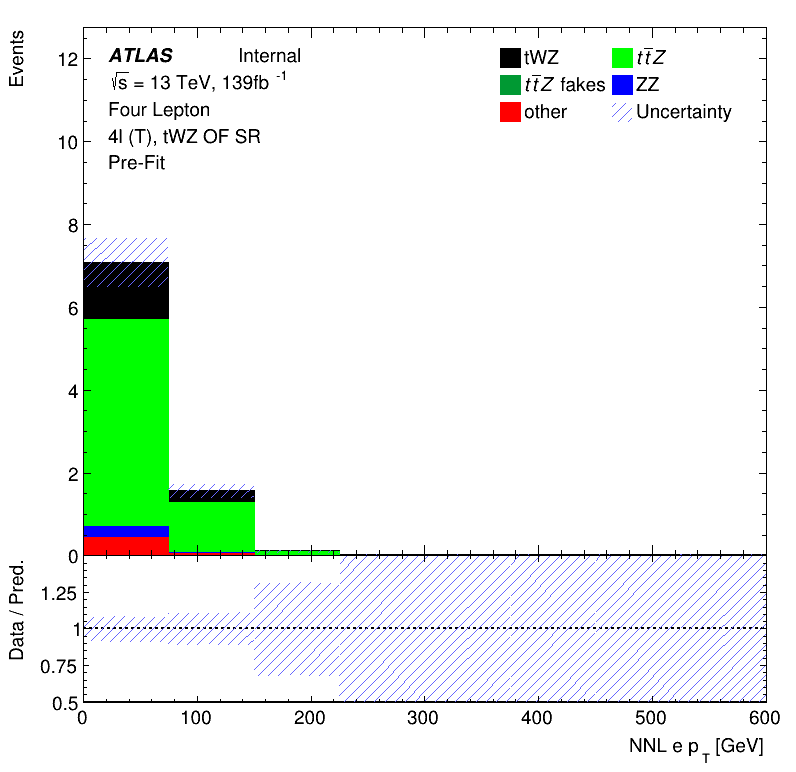
\includegraphics[width=.2\textwidth]{figures/PreFitPlots/lep4_tWZ_4T_OF_NNL_el_pt} & &
    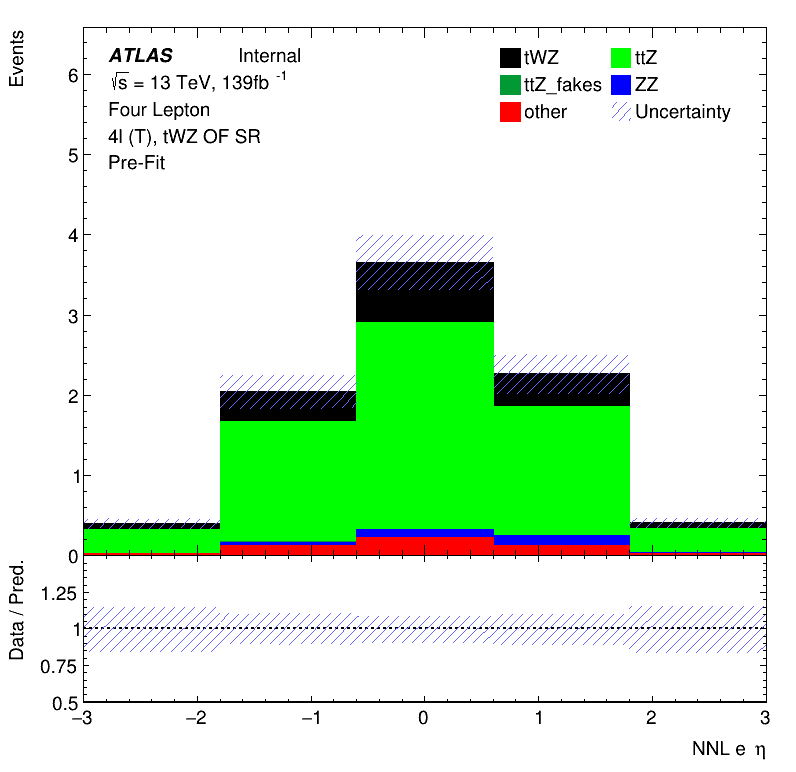
\includegraphics[width=.2\textwidth]{figures/PreFitPlots/lep4_tWZ_4T_OF_NNL_el_eta} \\
    \multicolumn{3}{c}{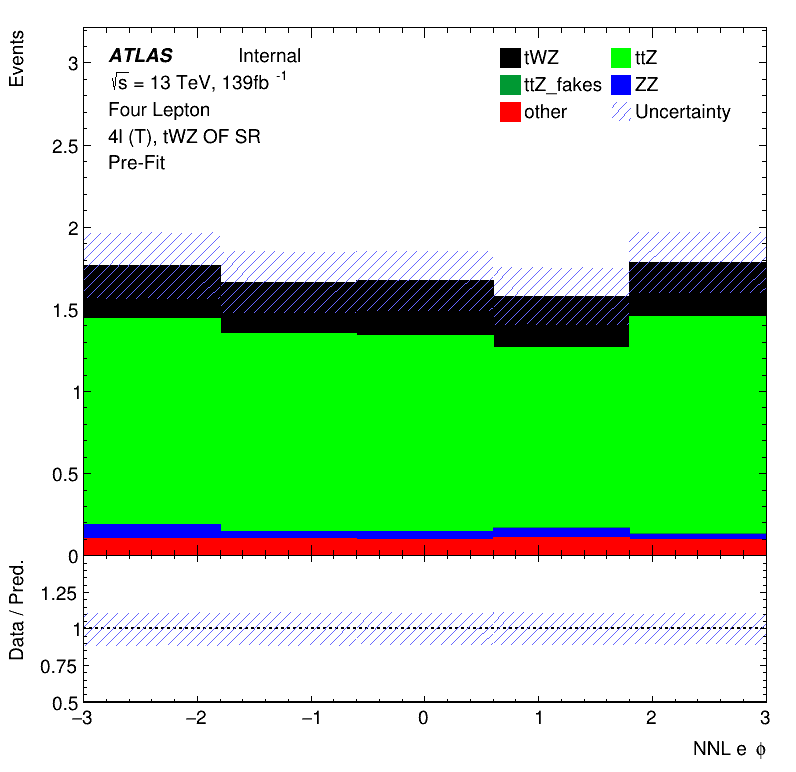
\includegraphics[width=.2\textwidth]{figures/PreFitPlots/lep4_tWZ_4T_OF_NNL_el_phi}}
  \end{tabular}
    \caption{MC predictions for $p_{T}$, $\eta$ (top row) and $\phi$ (bottom row) for next-to-next-to-leading (NNL) electrons in the $tWZ$ OF SR region}
  \label{fig:4lep-OF-SR-electronPlots}
\end{figure}


\begin{figure}[htbp]
    \centering
  \begin{tabular}{ccc}

    %%%%%%%%%%%%%%%%%
    %%%%% muons %%%%%
    %%%%%%%%%%%%%%%%%

    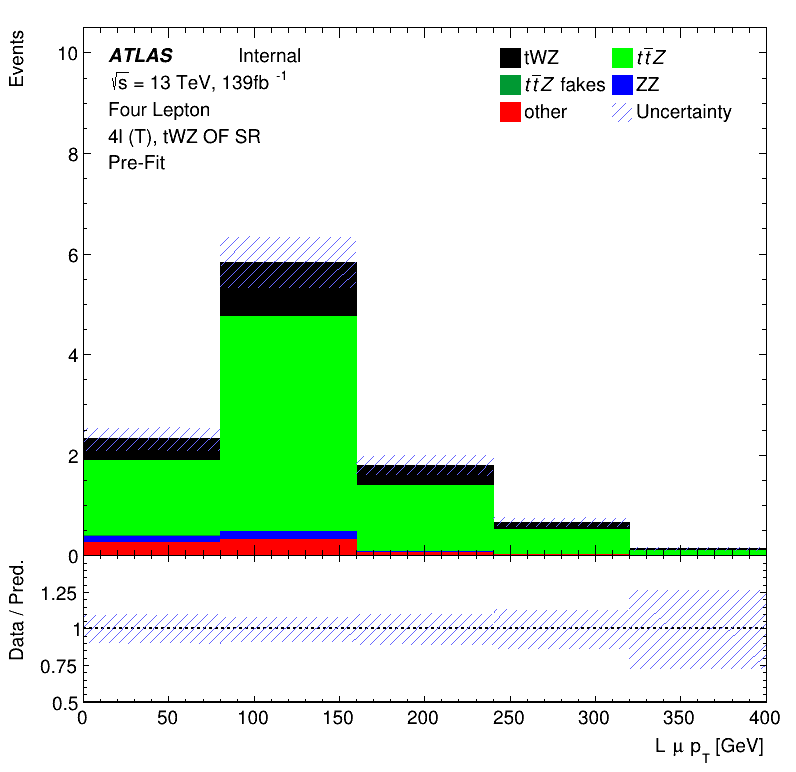
\includegraphics[width=.2\textwidth]{figures/PreFitPlots/lep4_tWZ_4T_OF_L_mu_pt} &
    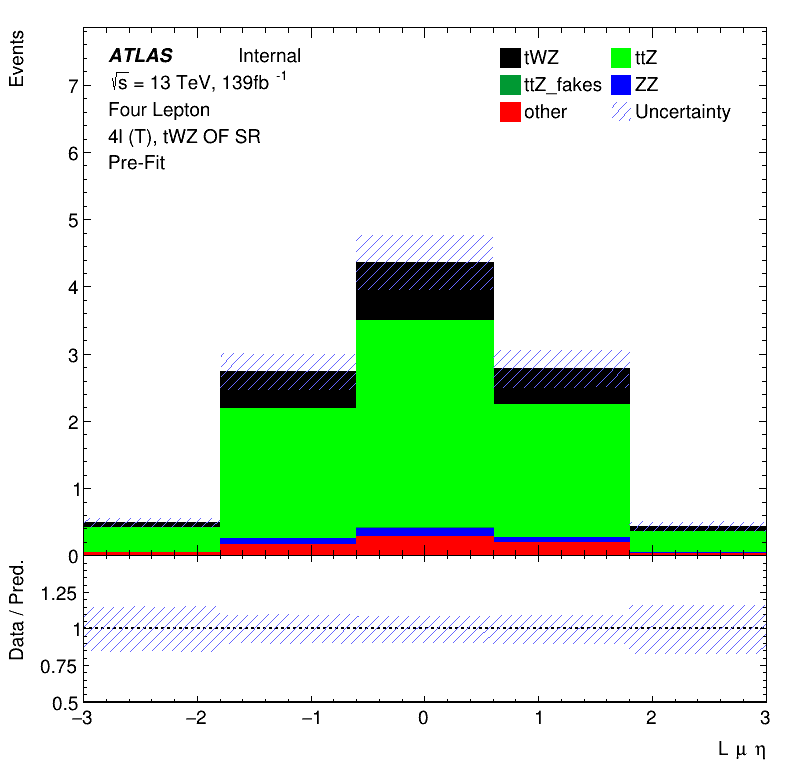
\includegraphics[width=.2\textwidth]{figures/PreFitPlots/lep4_tWZ_4T_OF_L_mu_eta} &
    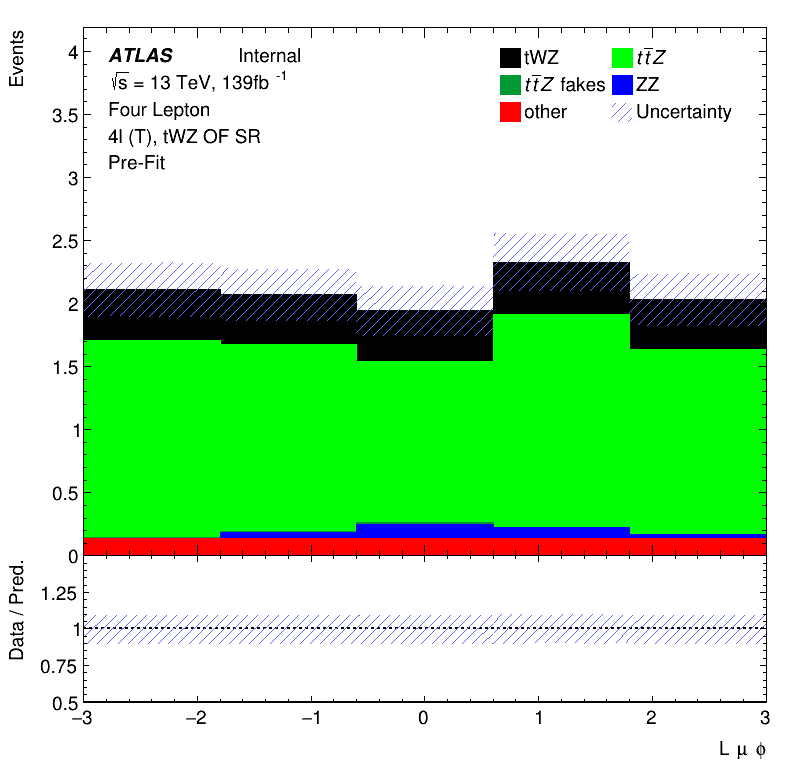
\includegraphics[width=.2\textwidth]{figures/PreFitPlots/lep4_tWZ_4T_OF_L_mu_phi} \\
    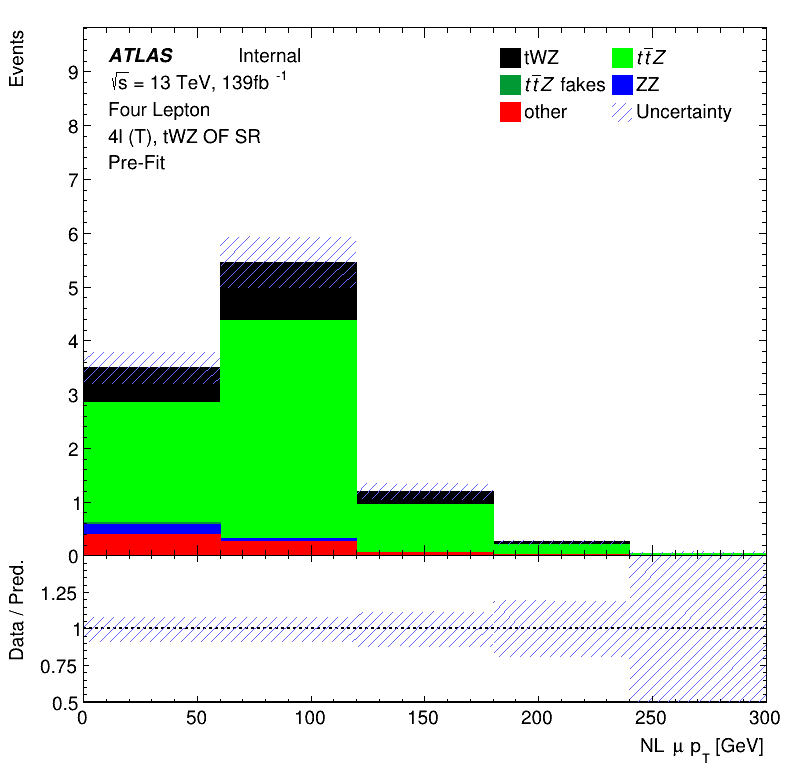
\includegraphics[width=.2\textwidth]{figures/PreFitPlots/lep4_tWZ_4T_OF_NL_mu_pt} &
    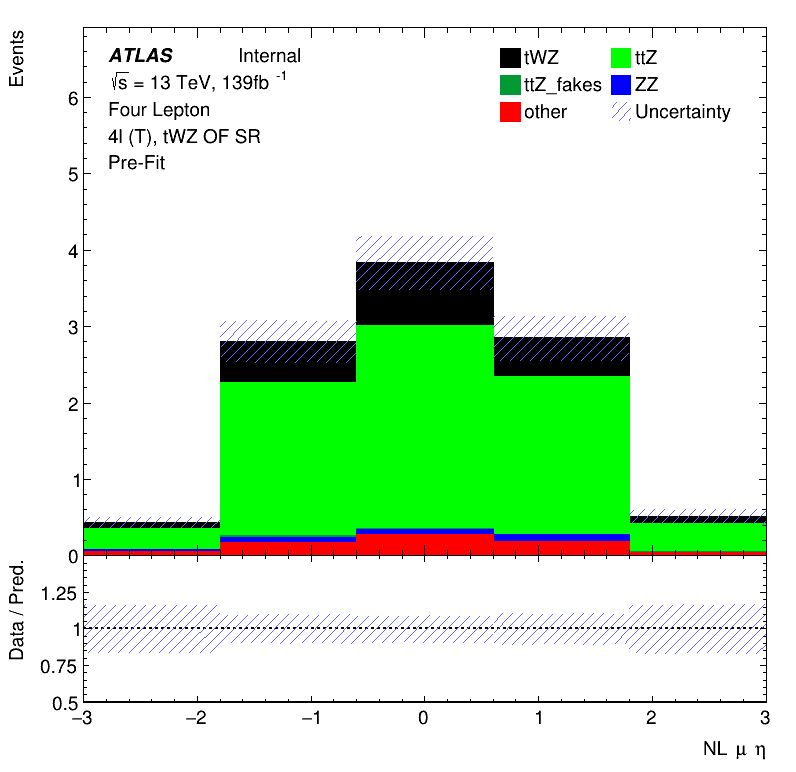
\includegraphics[width=.2\textwidth]{figures/PreFitPlots/lep4_tWZ_4T_OF_NL_mu_eta} &
    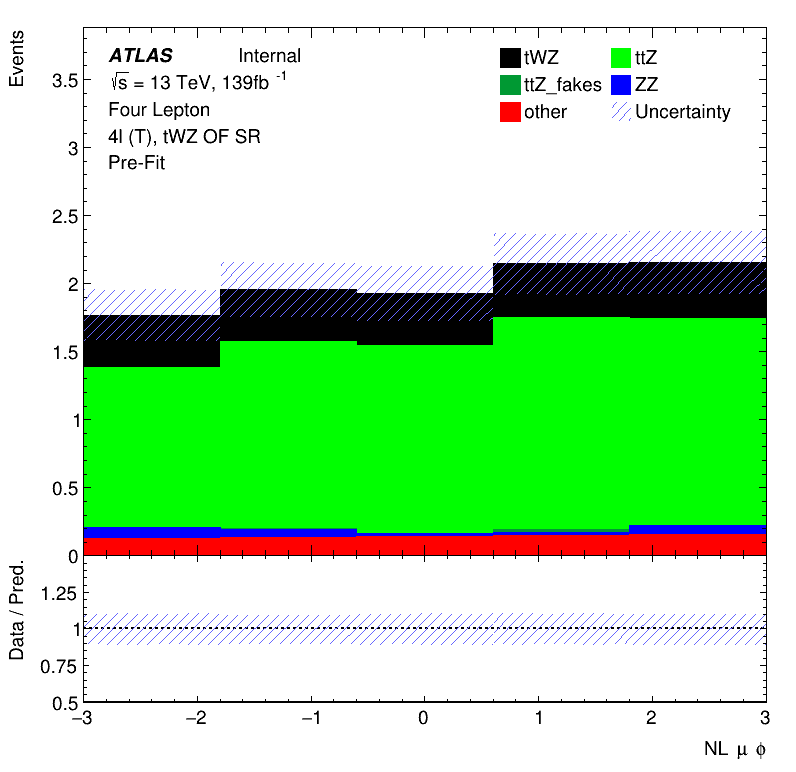
\includegraphics[width=.2\textwidth]{figures/PreFitPlots/lep4_tWZ_4T_OF_NL_mu_phi} \\

  \end{tabular}
    \caption{MC predictions for $p_{T}$, $\eta$ and $\phi$ for leading (L) muons (top row) and next-to-leading (NL) muons (bottom row) in the $tWZ$ OF SR region (\textit{blinded})}
\end{figure}
\clearpage

\begin{figure}[htbp]
\centering
  \begin{tabular}{ccc}

    %%%%%%%%%%%%%%%%%
    %%%%% muons %%%%%
    %%%%%%%%%%%%%%%%%


    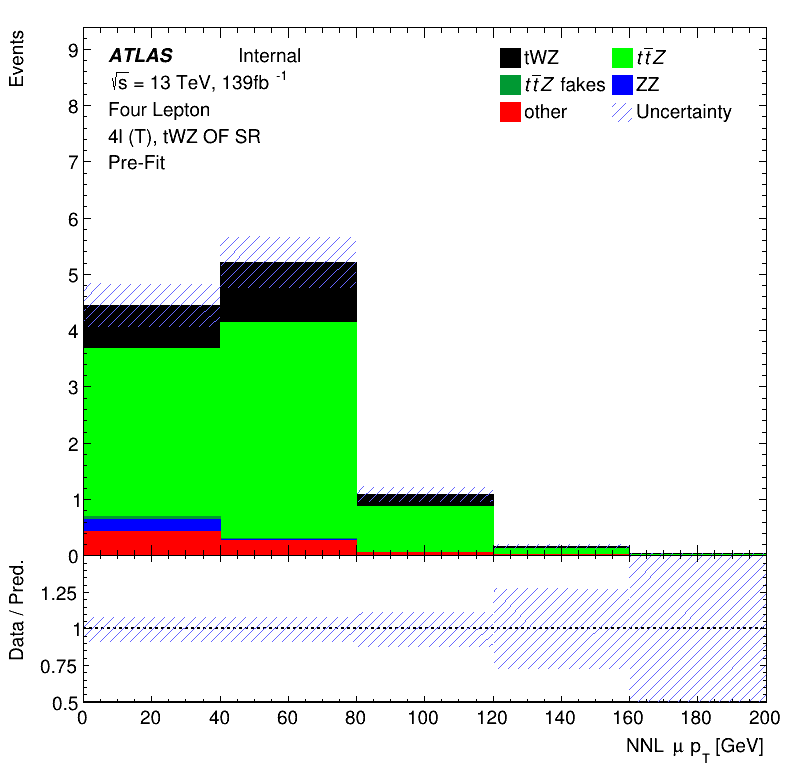
\includegraphics[width=.2\textwidth]{figures/PreFitPlots/lep4_tWZ_4T_OF_NNL_mu_pt} & &
    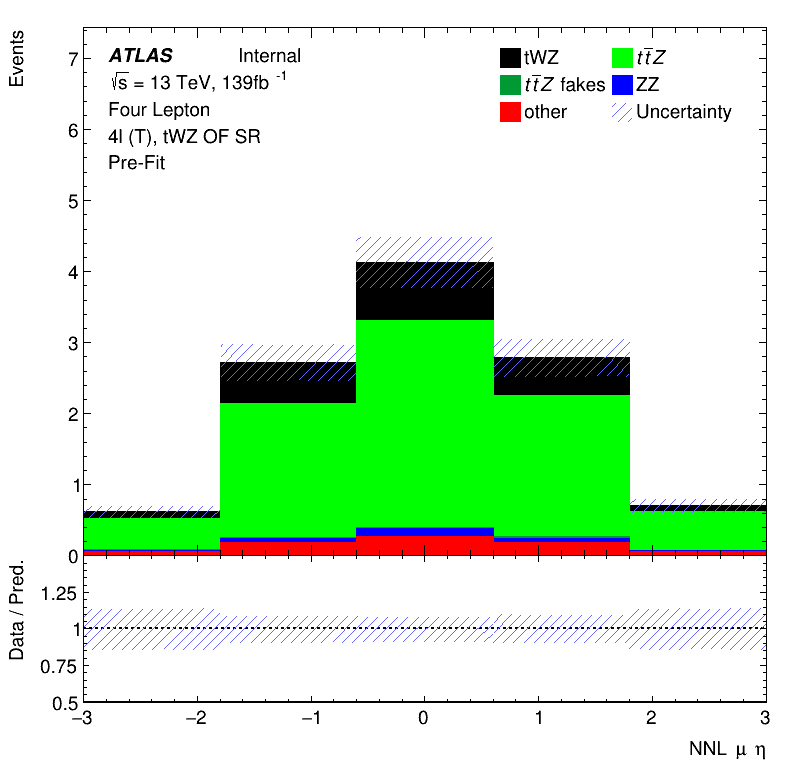
\includegraphics[width=.2\textwidth]{figures/PreFitPlots/lep4_tWZ_4T_OF_NNL_mu_eta}  \\
    \multicolumn{3}{c}{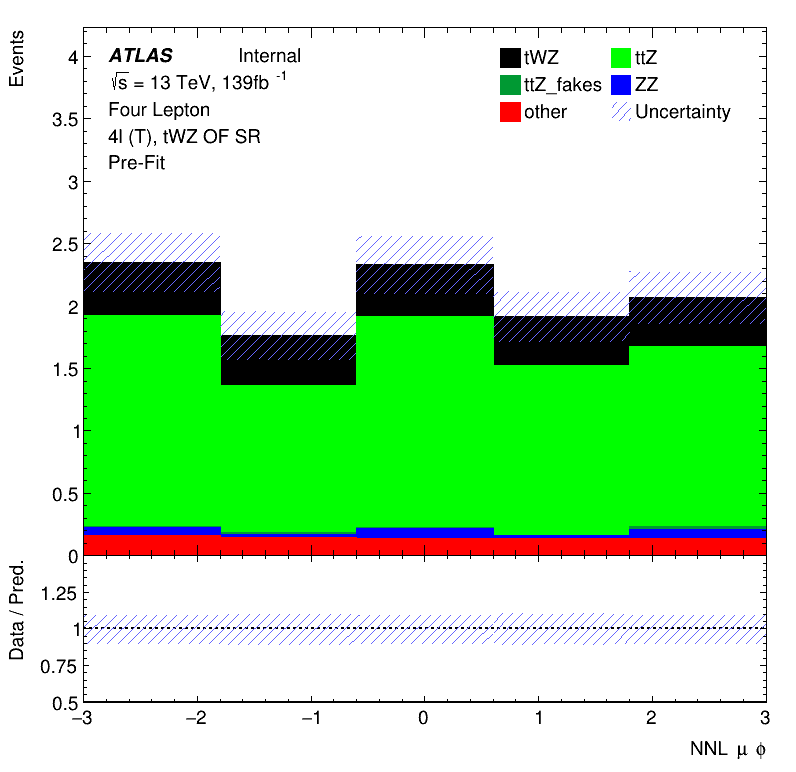
\includegraphics[width=.2\textwidth]{figures/PreFitPlots/lep4_tWZ_4T_OF_NNL_mu_phi}}  \\
  \end{tabular}
    \caption{MC predictions for $p_{T}$, $\eta$ (top row) and $\phi$ (bottom row) for next-to-next-to-leading (NNL) muons in the $tWZ$ OF SR region (\textit{blinded})}
  \label{fig:4lep-OF-SR-muonPlots}
\end{figure}

\begin{figure}[htbp]
\centering
  \begin{tabular}{ccc}
    %%%%%%%%%%%%%%%%%%%%%%%%%
    %%%%% untagged jets %%%%%
    %%%%%%%%%%%%%%%%%%%%%%%%%

    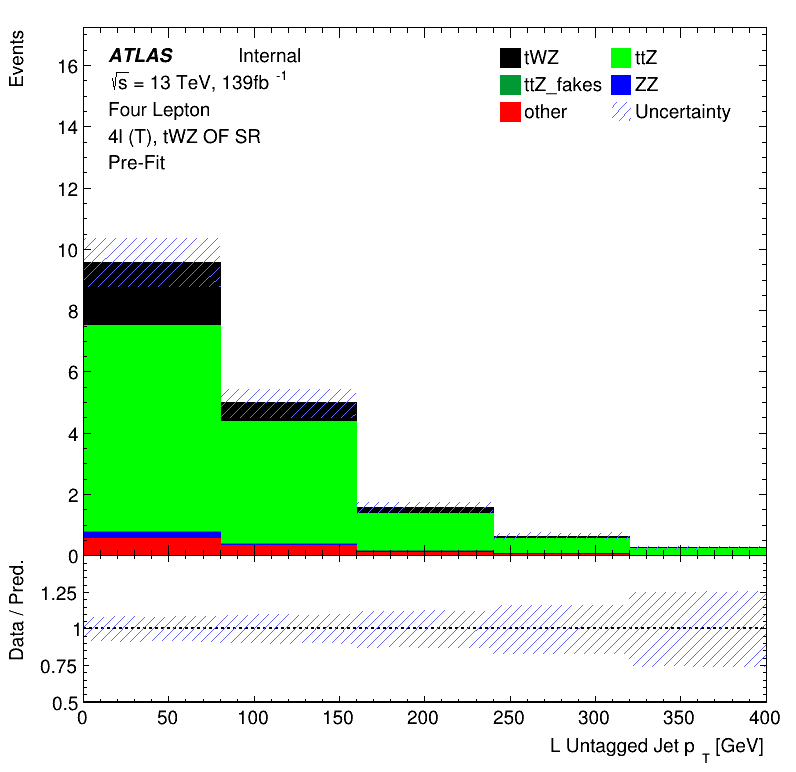
\includegraphics[width=.2\textwidth]{figures/PreFitPlots/lep4_tWZ_4T_OF_L_UntaggedJet_pt} & &
    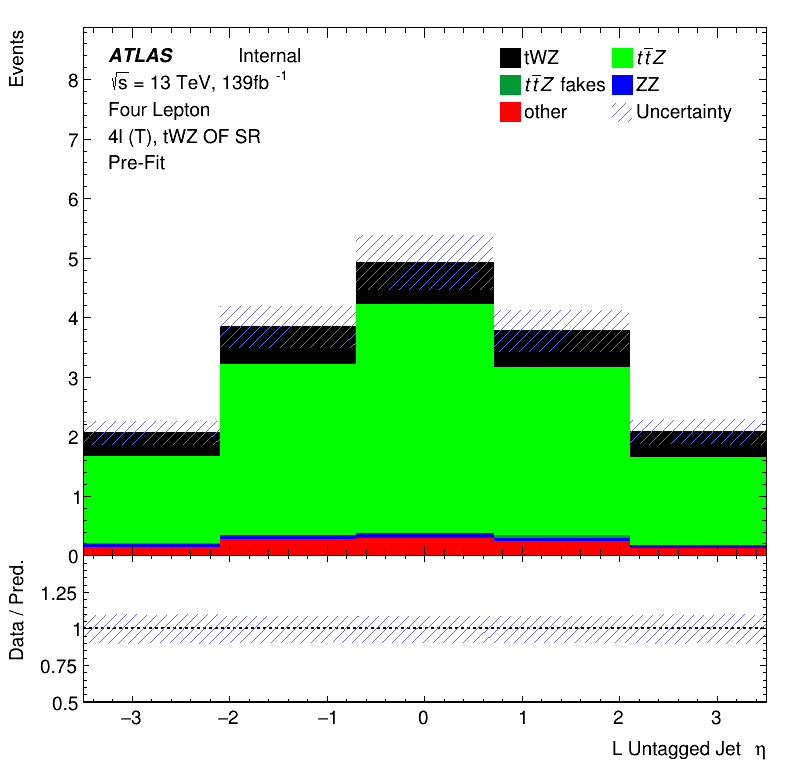
\includegraphics[width=.2\textwidth]{figures/PreFitPlots/lep4_tWZ_4T_OF_L_UntaggedJet_eta} \\
    \multicolumn{3}{c}{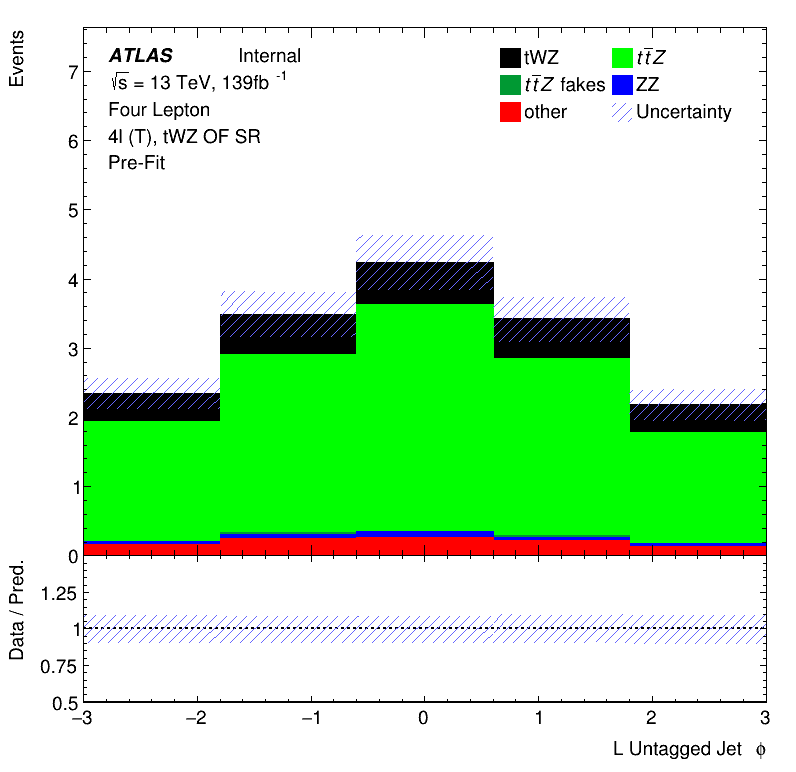
\includegraphics[width=.2\textwidth]{figures/PreFitPlots/lep4_tWZ_4T_OF_L_UntaggedJet_phi}}
  \end{tabular}
      \caption{MC predictions for $p_{T}$, $\eta$ (top row) and $\phi$ (bottom row) for untagged jets in the $tWZ$ OF SR region (\textit{blinded})}
  \label{fig:4lep-OF-SR-UntaggedjetPlots}
\end{figure}

\clearpage
\begin{figure}[htbp]
\centering
  \begin{tabular}{ccc}
    %%%%%%%%%%%%%%%%%%%%%%%%%
    %%%%% Z candidate %%%%%%%
    %%%%%%%%%%%%%%%%%%%%%%%%%

    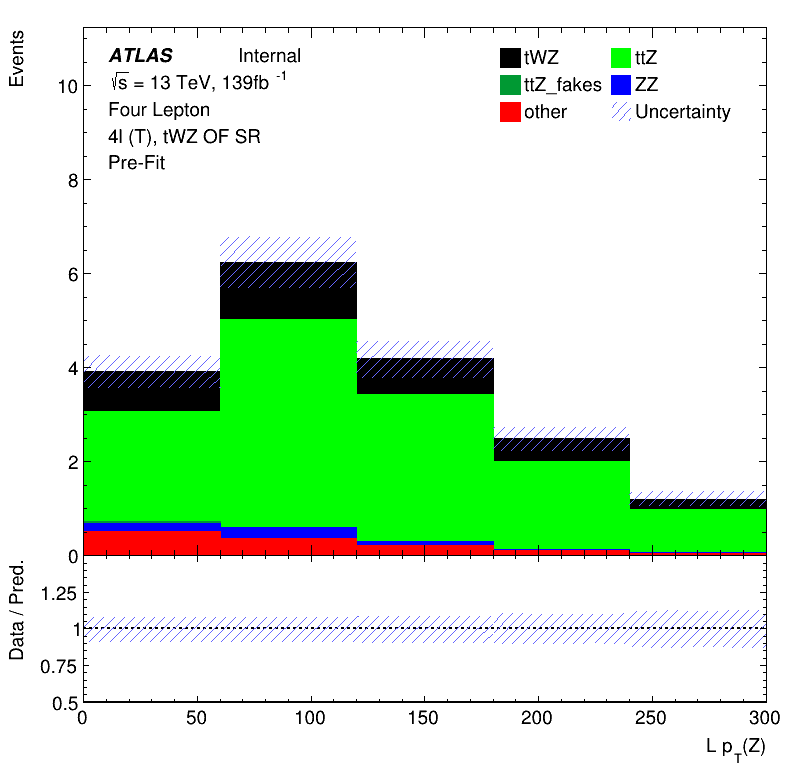
\includegraphics[width=.2\textwidth]{figures/PreFitPlots/lep4_tWZ_4T_OF_0_Z_pt}&
    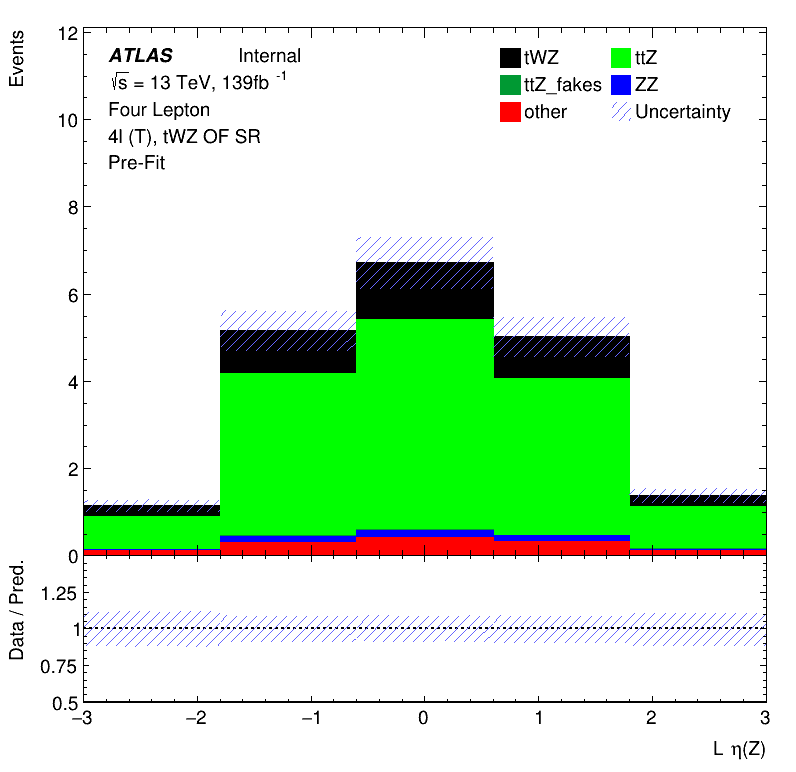
\includegraphics[width=.2\textwidth]{figures/PreFitPlots/lep4_tWZ_4T_OF_0_Z_eta} &
    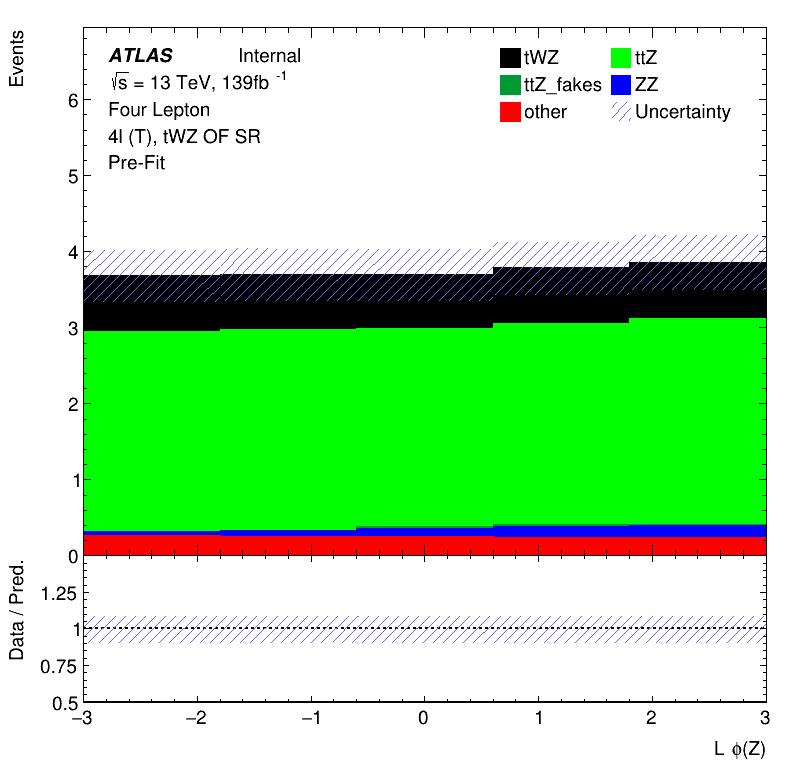
\includegraphics[width=.2\textwidth]{figures/PreFitPlots/lep4_tWZ_4T_OF_0_Z_phi} \\
    \multicolumn{3}{c}{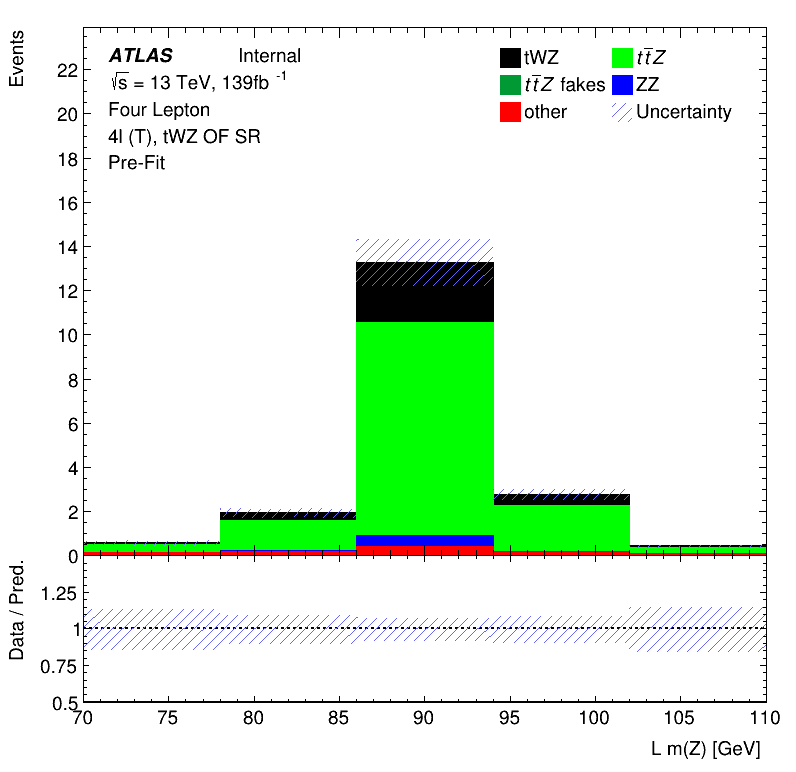
\includegraphics[width=.2\textwidth]{figures/PreFitPlots/lep4_tWZ_4T_OF_0_Z_mass}}

  \end{tabular}
    \caption{MC predictions for $p_{T}$, $\eta$, $\phi$ (top row) and mass ($m_Z$) (bottom row) of the leading reconstructed $Z$ candidate (OSSF lepton pair with $|m_{\text{OSSF}} - m(Z)| <  \SI{30}{\GeV}$) in the $tWZ$ OF SR region (\textit{blinded})}
  \label{fig:4lep-OF-SR-ZCands-Plots}
\end{figure}




\begin{figure}[htbp]
\centering
  \begin{tabular}{ccc}
    %%%%%%%%%%%%%%%%%%%%%%%%%%%
    %%%%% lepton system %%%%%%%
    %%%%%%%%%%%%%%%%%%%%%%%%%%%

    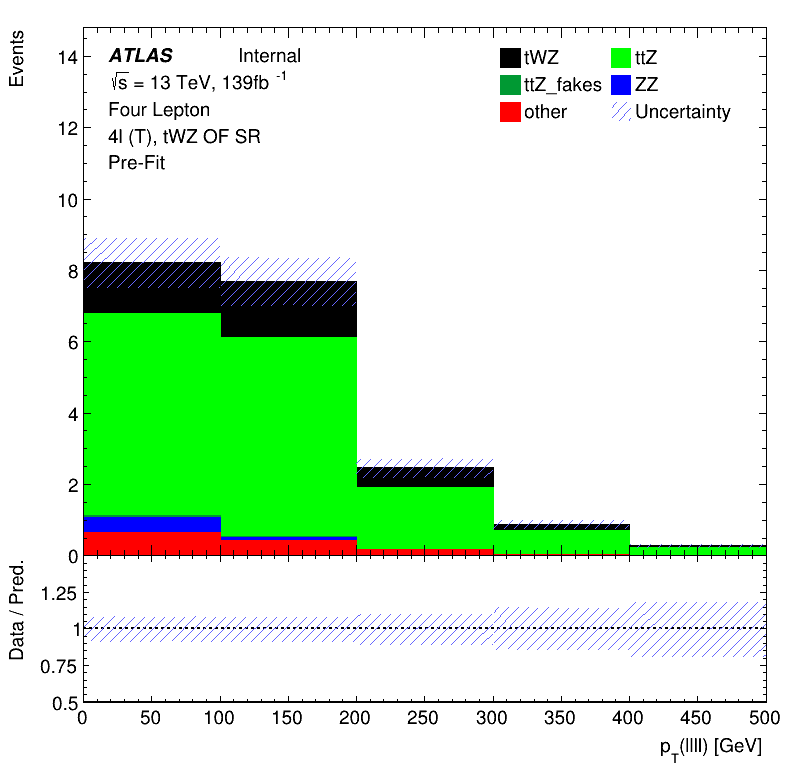
\includegraphics[width=.2\textwidth]{figures/PreFitPlots/lep4_tWZ_4T_OF_llll_sys_pt}&
    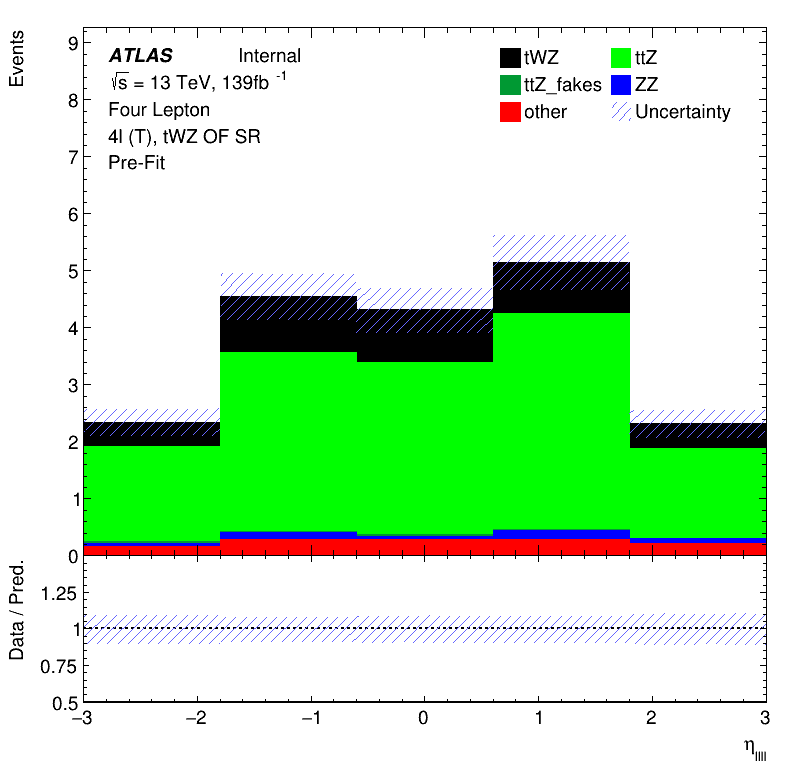
\includegraphics[width=.2\textwidth]{figures/PreFitPlots/lep4_tWZ_4T_OF_llll_sys_eta} &
    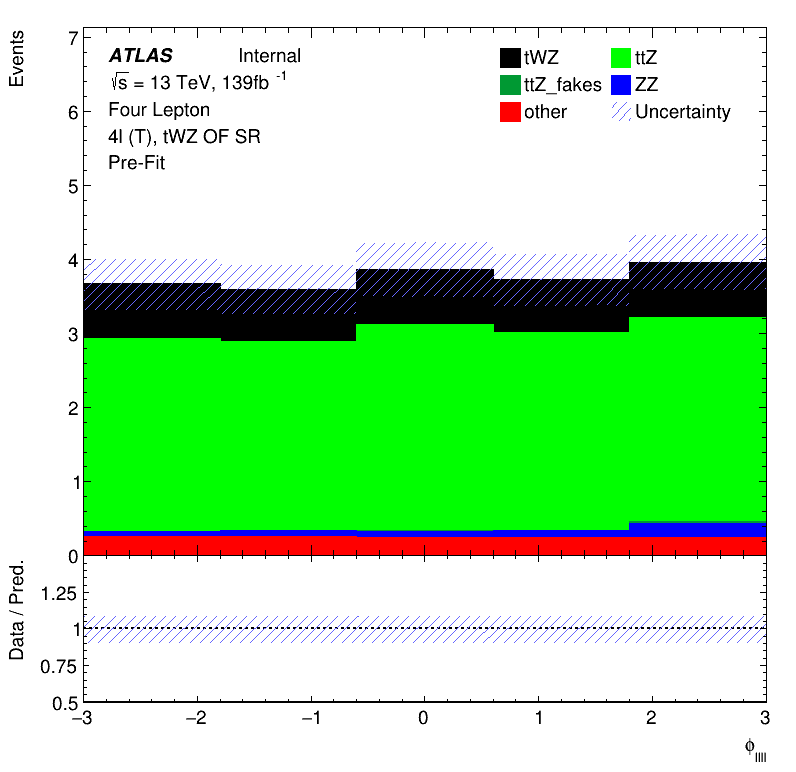
\includegraphics[width=.2\textwidth]{figures/PreFitPlots/lep4_tWZ_4T_OF_llll_sys_phi} \\
    \multicolumn{3}{c}{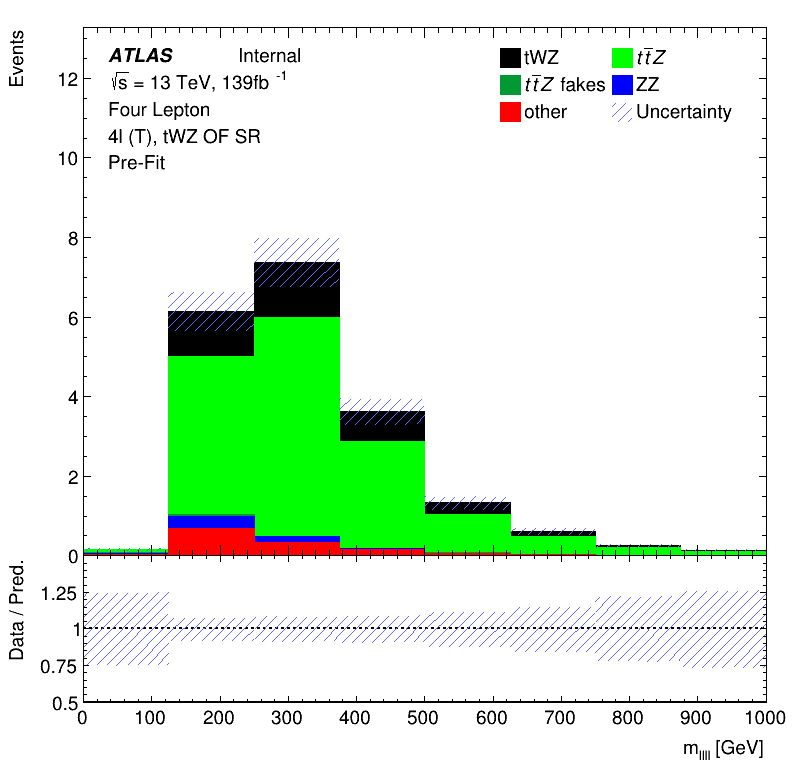
\includegraphics[width=.2\textwidth]{figures/PreFitPlots/lep4_tWZ_4T_OF_llll_sys_mass}}

  \end{tabular}
  \caption{MC predictions for $p_{T}$, $\eta$, $\phi$ (top row) and mass (bottom row) of the lepton system ($\ell \ell \ell \ell$) in the $tWZ$ OF SR region (\textit{blinded})}
  \label{fig:4lep-OF-SR-Lep-sys-Plots}
\end{figure}
\clearpage

\begin{figure}[htbp]
\centering
  \begin{tabular}{ccc}
    %%%%%%%%%%%%%%%%%%%%%%%%%%%
    %%%%%    jet system %%%%%%%
    %%%%%%%%%%%%%%%%%%%%%%%%%%%

    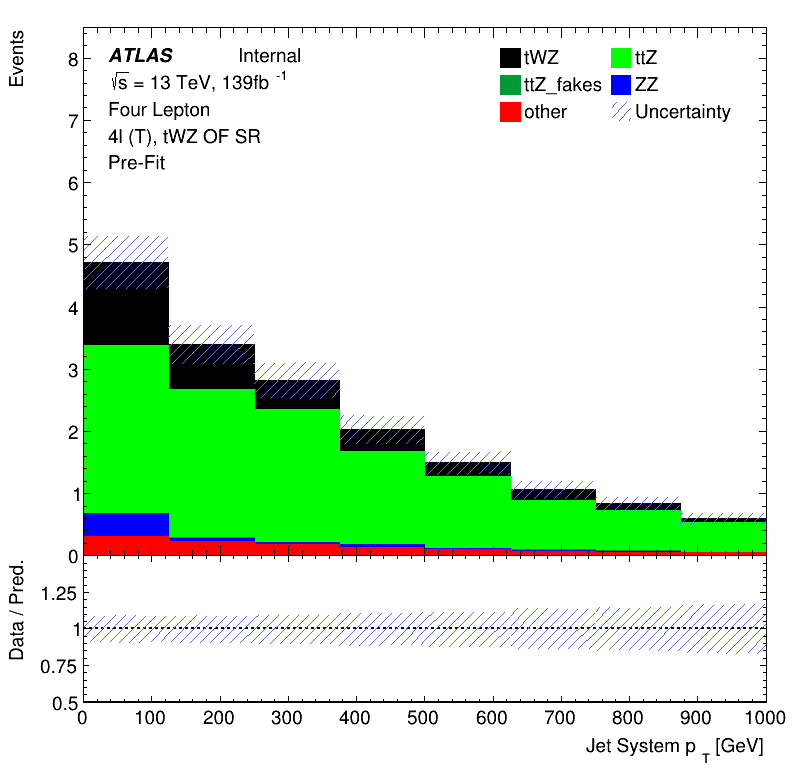
\includegraphics[width=.2\textwidth]{figures/PreFitPlots/lep4_tWZ_4T_OF_Jet_sys_Pt}&
    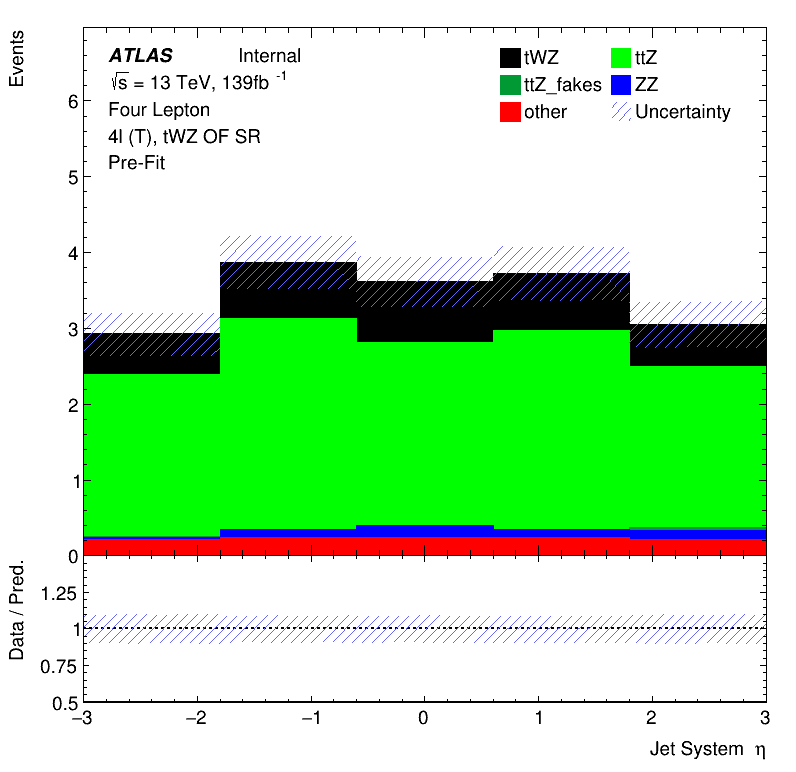
\includegraphics[width=.2\textwidth]{figures/PreFitPlots/lep4_tWZ_4T_OF_Jet_sys_Eta} &
    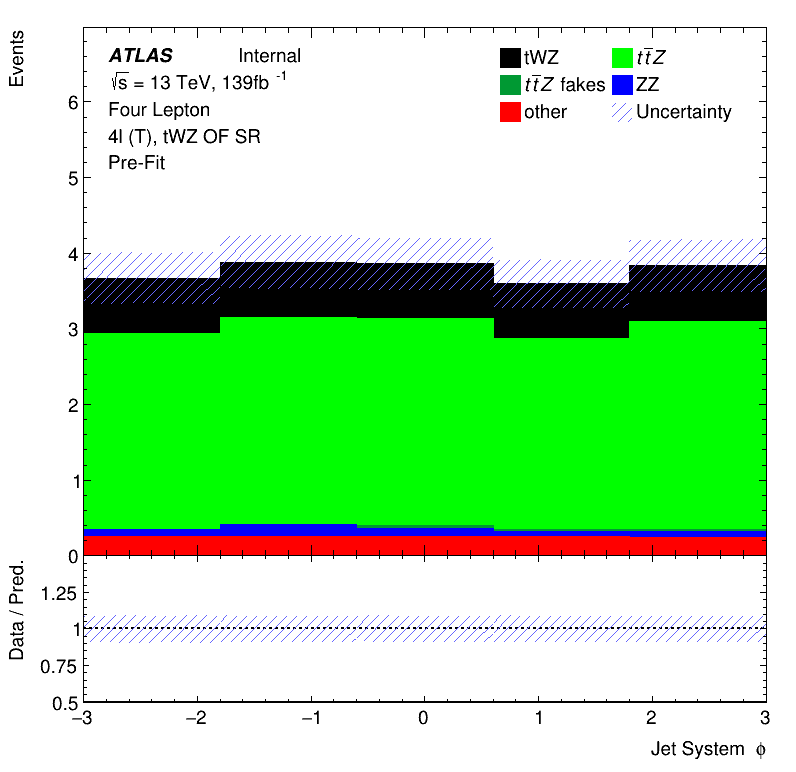
\includegraphics[width=.2\textwidth]{figures/PreFitPlots/lep4_tWZ_4T_OF_Jet_sys_Phi} \\
    \multicolumn{3}{c}{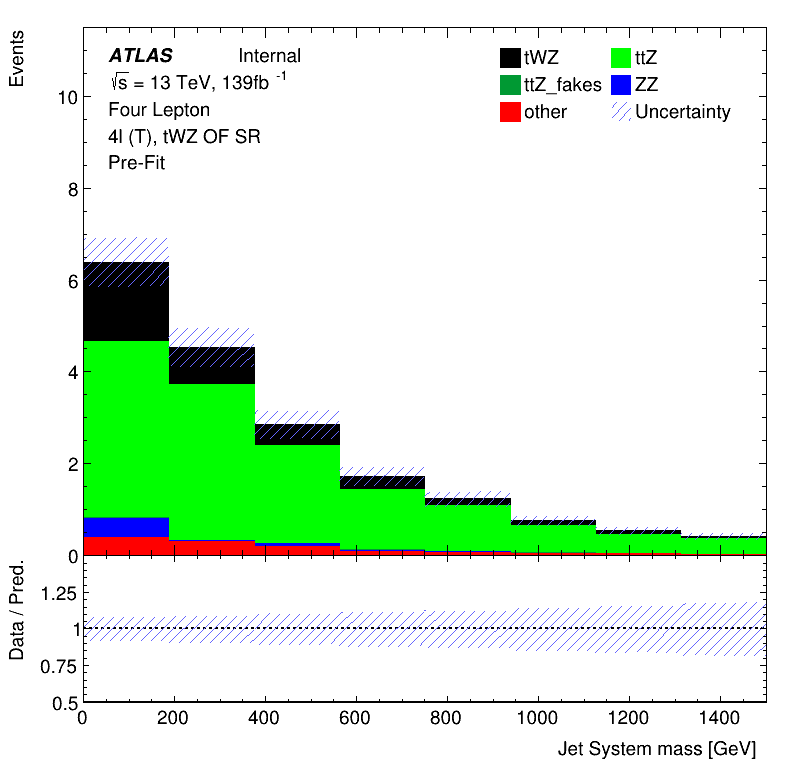
\includegraphics[width=.2\textwidth]{figures/PreFitPlots/lep4_tWZ_4T_OF_Jet_sys_mass}}

  \end{tabular}
  \caption{MC predictions for $p_{T}$, $\eta$, $\phi$ (top row) and mass (bottom row) of the jet systems in the $tWZ$ OF SR region (\textit{blinded})}
  \label{fig:4lep-OF-SR-jet-sys-Plots}
\end{figure}


\begin{figure}[htbp]
\centering
  \begin{tabular}{ccc}
    %%%%%%%%%%%%%%%%%%%%%%%%%%%
    %%%%%   b jet system %%%%%%
    %%%%%%%%%%%%%%%%%%%%%%%%%%%

    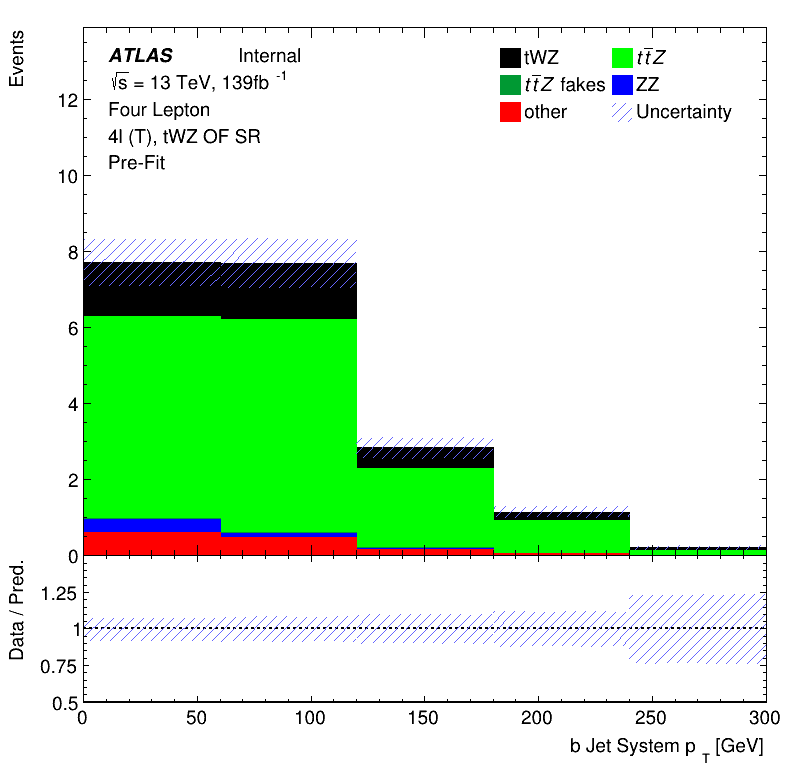
\includegraphics[width=.2\textwidth]{figures/PreFitPlots/lep4_tWZ_4T_OF_bJet_sys_Pt}&
    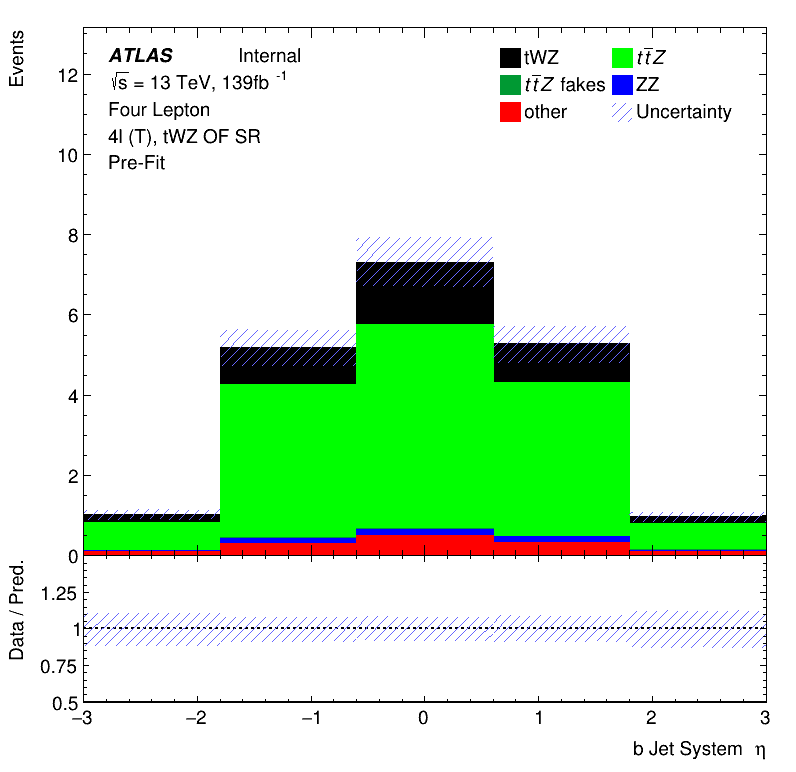
\includegraphics[width=.2\textwidth]{figures/PreFitPlots/lep4_tWZ_4T_OF_bJet_sys_Eta} &
    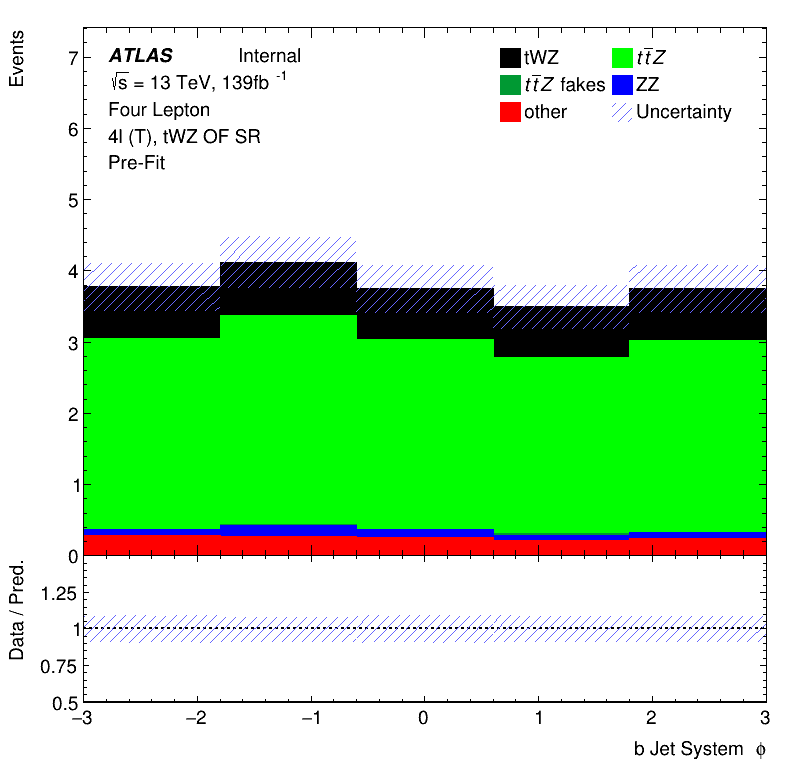
\includegraphics[width=.2\textwidth]{figures/PreFitPlots/lep4_tWZ_4T_OF_bJet_sys_Phi} \\
    \multicolumn{3}{c}{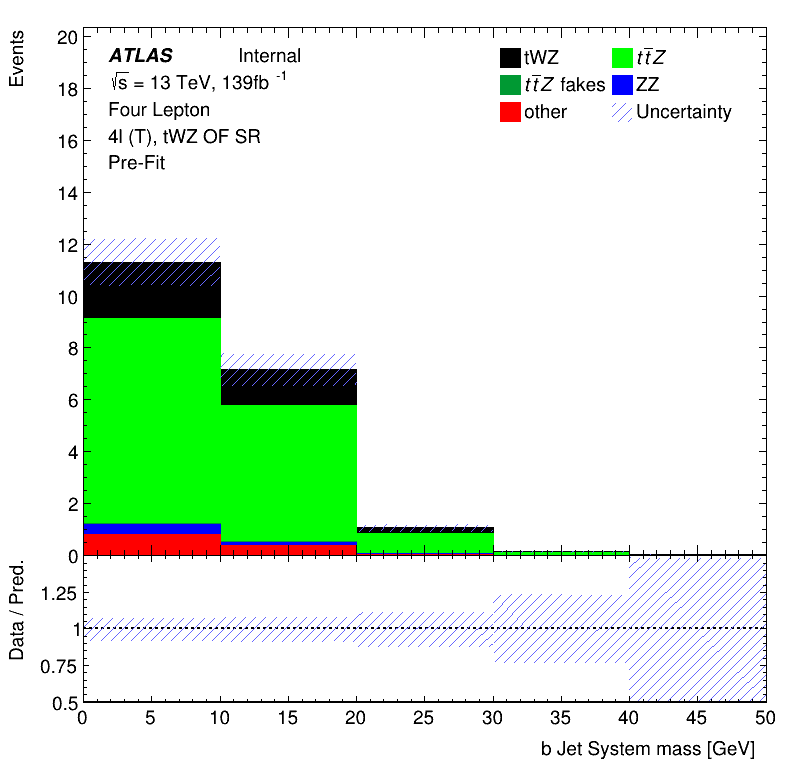
\includegraphics[width=.2\textwidth]{figures/PreFitPlots/lep4_tWZ_4T_OF_bJet_sys_mass}}

  \end{tabular}
  \caption{MC predictions for $p_{T}$, $\eta$, $\phi$ (top row) and mass (bottom row) of the b-tagged jet systems in the $tWZ$ OF SR region (\textit{blinded})}
  \label{fig:4lep-OF-SR-bjet-sys-Plots}
\end{figure}
\clearpage

\begin{figure}[htbp]
\centering

    %%%%%%%%%%%%%%%%%%%%%%%%%%%%%%%%
    %%%%% jets and leps system %%%%%
    %%%%%%%%%%%%%%%%%%%%%%%%%%%%%%%%
    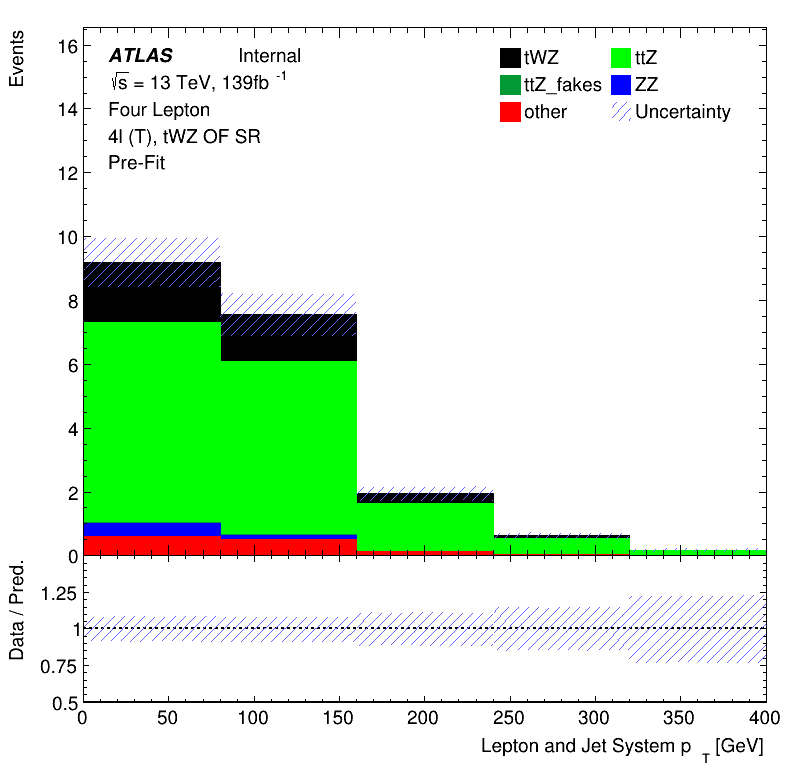
\includegraphics[width=.2\textwidth]{figures/PreFitPlots/lep4_tWZ_4T_OF_Jets_Leps_sys_Pt}\quad
    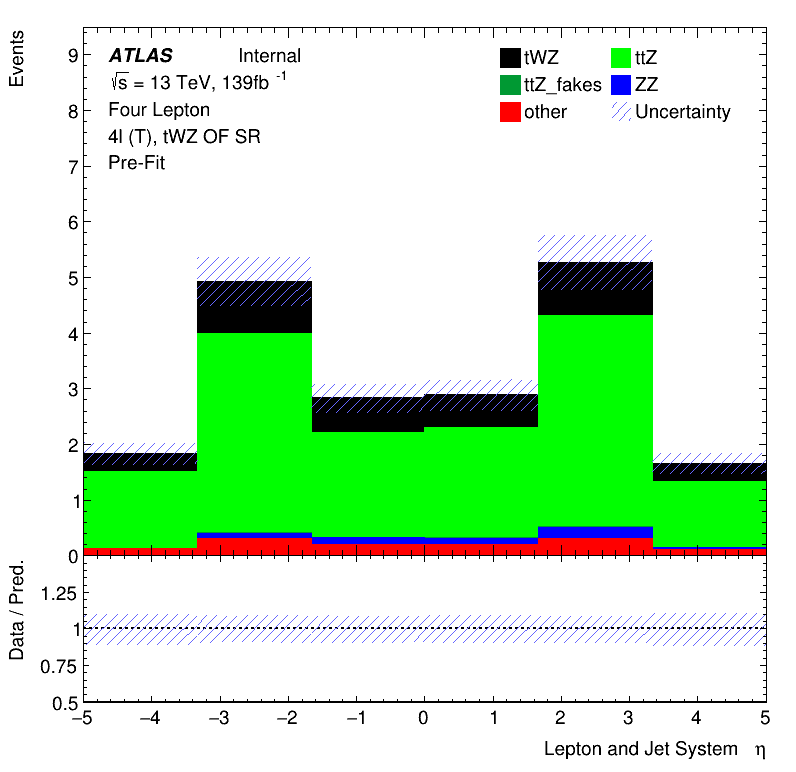
\includegraphics[width=.2\textwidth]{figures/PreFitPlots/lep4_tWZ_4T_OF_Jets_Leps_sys_eta} \quad
    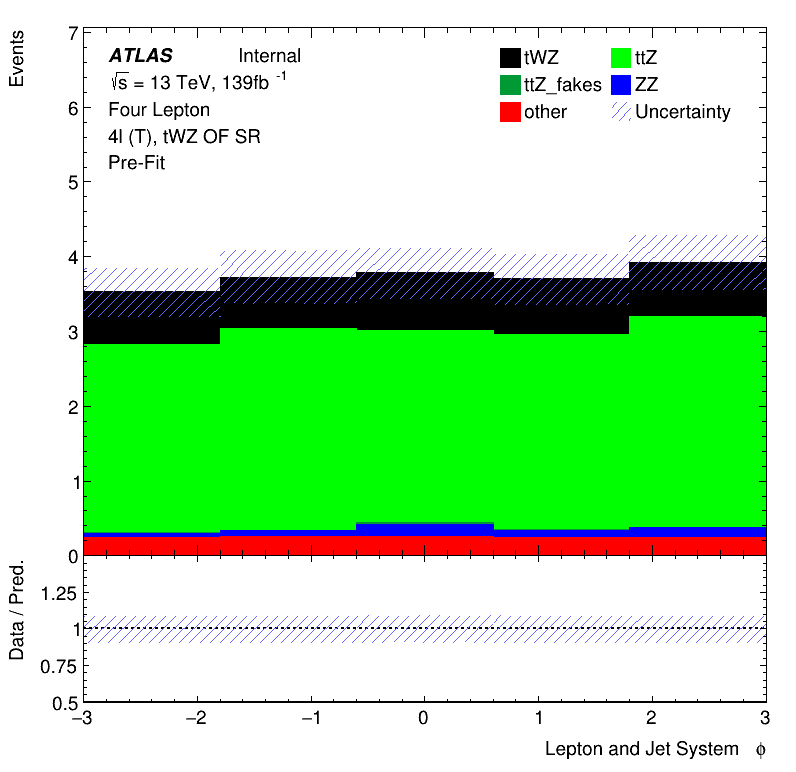
\includegraphics[width=.2\textwidth]{figures/PreFitPlots/lep4_tWZ_4T_OF_Jets_Leps_sys_phi}
    \medskip
    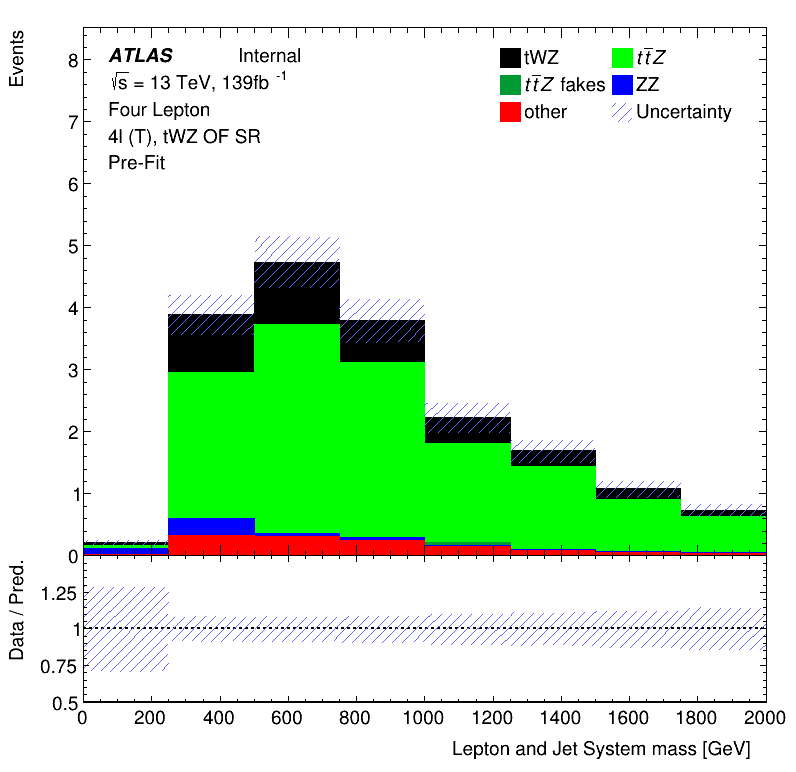
\includegraphics[width=.2\textwidth]{figures/PreFitPlots/lep4_tWZ_4T_OF_Jets_Leps_sys_mass} \quad
    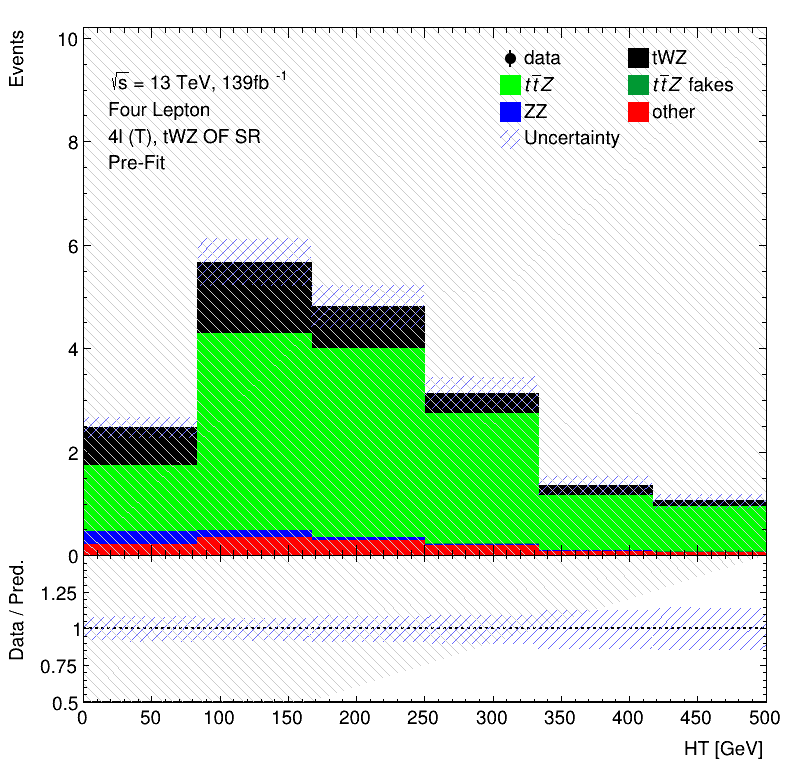
\includegraphics[width=.2\textwidth]{figures/PreFitPlots/lep4_tWZ_4T_OF_HT}

\caption{MC predictions for $p_{T}$, $\eta$ and $\phi$ (top row) and mass (bottom left) for the lepton $+$ jet systems ($\ell \ell \ell \ell + $ jets) in the $tWZ$ OF SR region (\textit{blinded}). Bottom right: MC predictions for $H_{T}$ (scalar sum of jet $p_{T}$ and lepton $p_{T}$) in the $tWZ$ OF SR region (\textit{blinded})}
  \label{fig:4lep-OF-SR-jets-and-leps-sys-Plots}
\end{figure}


\begin{figure}[htbp]
\centering
  \begin{tabular}{ccc}
    %%%%%%%%%%%%%%%%%%%%%%%%%%%%%%%%%%%%
    %%%%%   b jet and leps system %%%%%%
    %%%%%%%%%%%%%%%%%%%%%%%%%%%%%%%%%%%%

    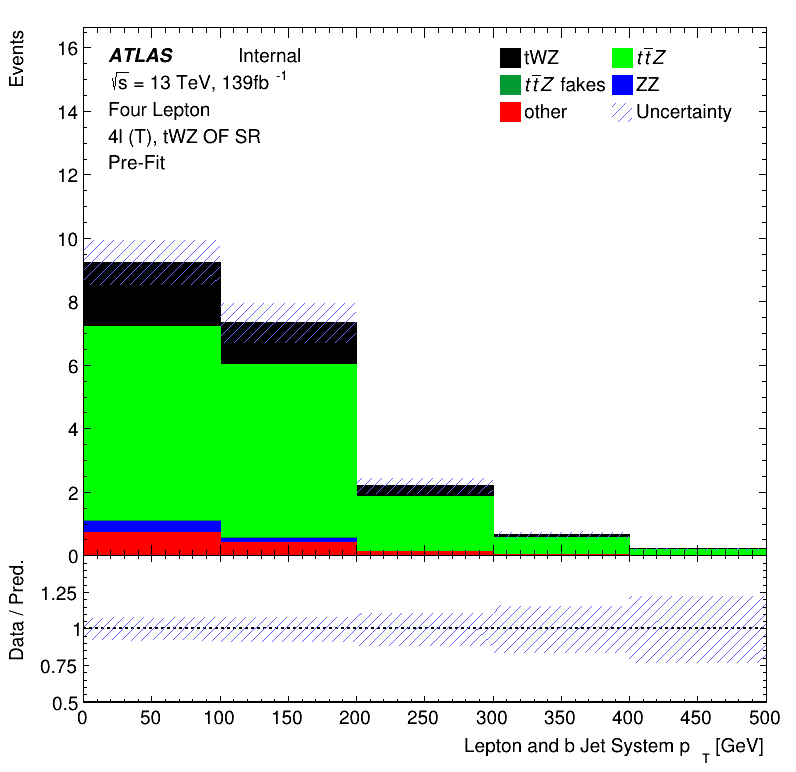
\includegraphics[width=.2\textwidth]{figures/PreFitPlots/lep4_tWZ_4T_OF_bJets_Leps_sys_pt}&
    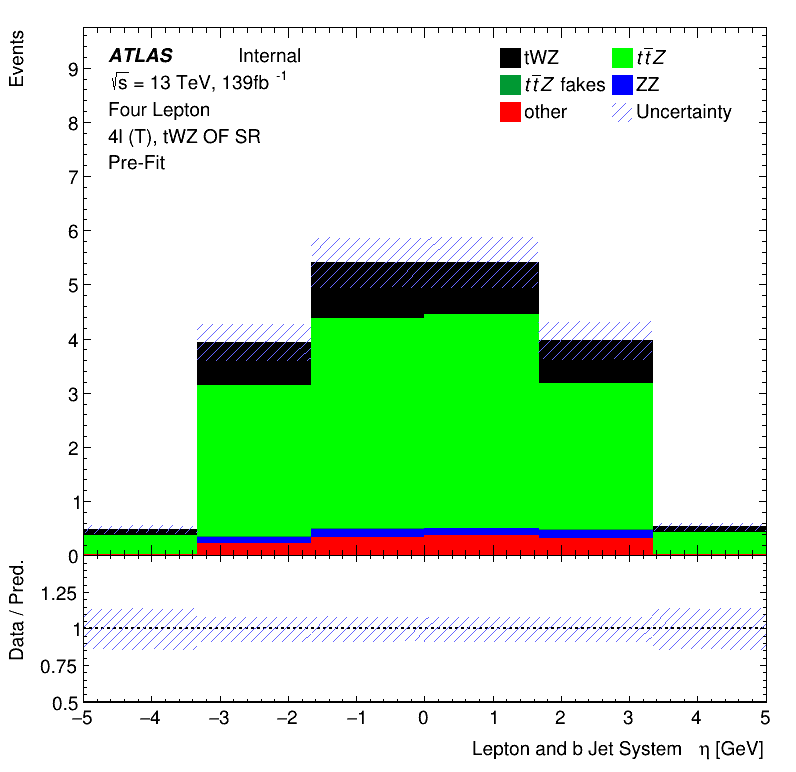
\includegraphics[width=.2\textwidth]{figures/PreFitPlots/lep4_tWZ_4T_OF_bJets_Leps_sys_eta} &
    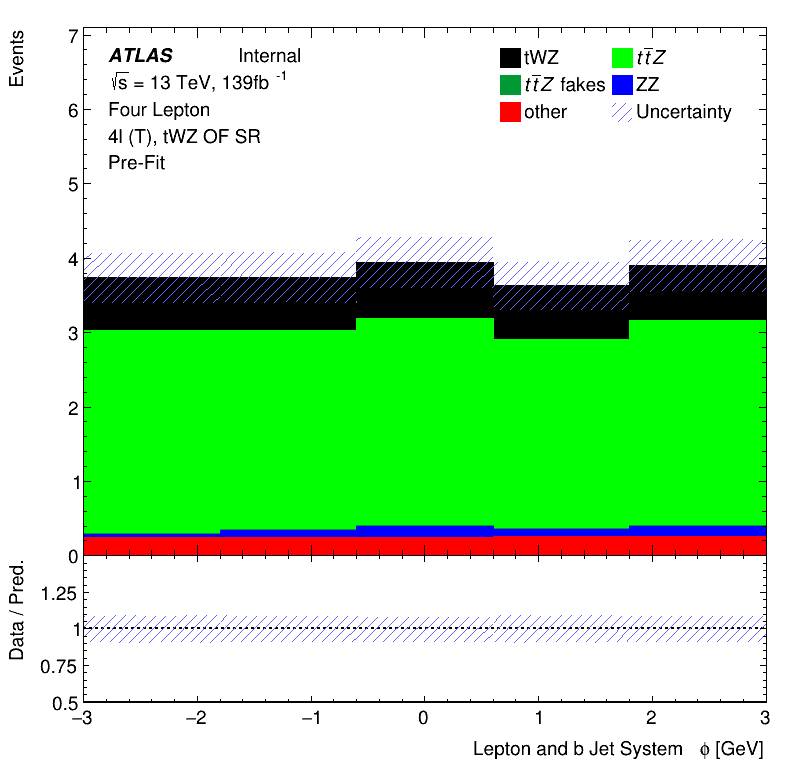
\includegraphics[width=.2\textwidth]{figures/PreFitPlots/lep4_tWZ_4T_OF_bJets_Leps_sys_phi} \\
    \multicolumn{3}{c}{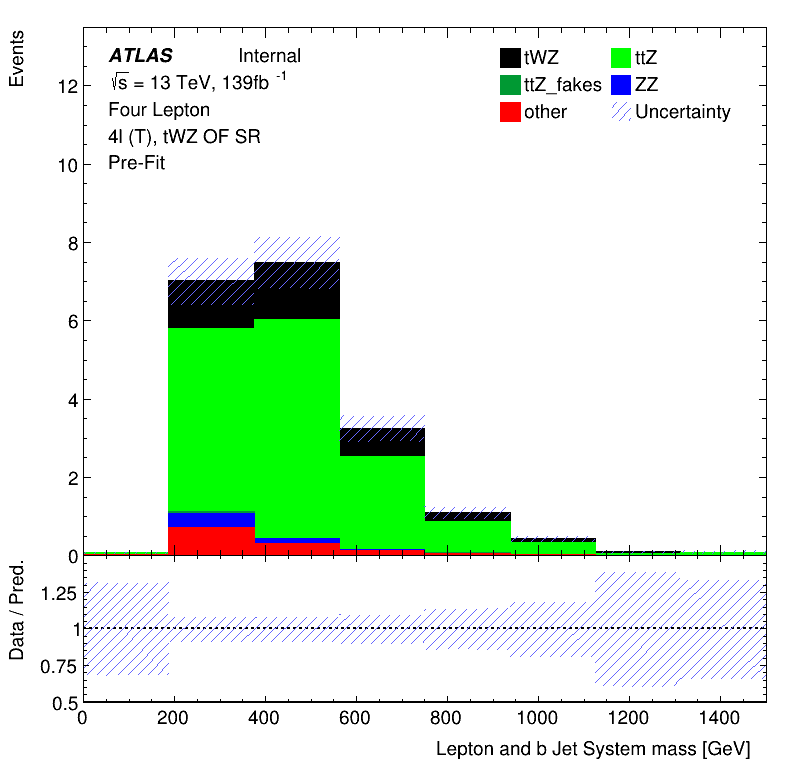
\includegraphics[width=.2\textwidth]{figures/PreFitPlots/lep4_tWZ_4T_OF_bJets_Leps_sys_mass}}

  \end{tabular}
    \caption{MC predictions for $p_{T}$, $\eta$, $\phi$ (top row) and mass (bottom row) of the lepton $+$ b-tagged jet systems ($\ell \ell \ell \ell + $ b-tagged jets) in the $tWZ$ OF SR region (\textit{blinded})}
  \label{fig:4lep-OF-SR-bjet-and-leps-sys-Plots}
\end{figure}
\clearpage

\begin{figure}[htbp]
\centering
  \begin{tabular}{ccc}
    %%%%%%%%%%%%%%%%%%%%%%%%%%%%%%%%%%%%
    %%%%%  non Z leps system      %%%%%%
    %%%%%%%%%%%%%%%%%%%%%%%%%%%%%%%%%%%%

    \includegraphics[width=.2\textwidth]{figures/PreFitPlots/lep4_tWZ_4T_OF_nonZll_sys_pt}&
    \includegraphics[width=.2\textwidth]{figures/PreFitPlots/lep4_tWZ_4T_OF_nonZll_sys_eta} &
    \includegraphics[width=.2\textwidth]{figures/PreFitPlots/lep4_tWZ_4T_OF_nonZll_sys_phi} \\
    \multicolumn{3}{c}{\includegraphics[width=.2\textwidth]{figures/PreFitPlots/lep4_tWZ_4T_OF_nonZll_sys_mass}}

  \end{tabular}
      \caption{MC predictions for $p_{T}$, $\eta$, $\phi$ (top row) and mass (bottom row) of reconstructed Non $Z$ leptons (lepton pairs which don't originate from a $Z$ candiate) in the $tWZ$ OF SR region (\textit{blinded})}
  \label{fig:4lep-OF-SR-NonZLeps-sys-Plots}
\end{figure}



\subsection{$tWZ$ SF SR}
\label{sec:app-controlplotstetralepton-tWZ-SF-SR}

\begin{figure}[htbp]
  \centering
  \begin{tabular}{ccc}

    %%%%%%%%%%%%%%%
    %%% Leptons %%%
    %%%%%%%%%%%%%%%


    \includegraphics[width=.2\textwidth]{figures/PreFitPlots/lep4_tWZ_4T_SF_NNL_lepton_pt} &
    \includegraphics[width=.2\textwidth]{figures/PreFitPlots/lep4_tWZ_4T_SF_NNL_lepton_eta} &
    \includegraphics[width=.2\textwidth]{figures/PreFitPlots/lep4_tWZ_4T_SF_NNL_lepton_phi} \\
    \multicolumn{3}{c}{\includegraphics[width=.2\textwidth]{figures/PreFitPlots/lep4_tWZ_4T_SF_LT} }\\

  \end{tabular}
  \caption{Top row: MC predictions for $p_{T}$, $\eta$ and $\phi$ for next-to-next-to-leading (NNL) leptons in the $tWZ$ SF SR region (\textit{blinded}). Bottom row: MC predictions for $L_{T}$ (scalar sum of lepton $p_{T}$)  in the $tWZ$ SF SR region (\textit{blinded})}
  \label{fig:4lep-SF-SR-leptonPlots}
\end{figure}


\begin{figure}[htbp]
  \centering
  \begin{tabular}{ccc}
    %%%%%%%%%%%%%%%%%
    %%% electrons %%%
    %%%%%%%%%%%%%%%%%


    \includegraphics[width=.2\textwidth]{figures/PreFitPlots/lep4_tWZ_4T_SF_L_el_pt} &
    \includegraphics[width=.2\textwidth]{figures/PreFitPlots/lep4_tWZ_4T_SF_L_el_eta} &
    \includegraphics[width=.2\textwidth]{figures/PreFitPlots/lep4_tWZ_4T_SF_L_el_phi} \\
    \includegraphics[width=.2\textwidth]{figures/PreFitPlots/lep4_tWZ_4T_SF_NL_el_pt} &
    \includegraphics[width=.2\textwidth]{figures/PreFitPlots/lep4_tWZ_4T_SF_NL_el_eta} &
    \includegraphics[width=.2\textwidth]{figures/PreFitPlots/lep4_tWZ_4T_SF_NL_el_phi} \\

  \end{tabular}
    \caption{MC predictions for $p_{T}$, $\eta$ and $\phi$ for leading (L) electrons (top row) and next-to-leading (NL) electrons (bottom row) in the $tWZ$ SF SR region (\textit{blinded})}
  \label{fig:4lep-SF-SR-electronPlots}
\end{figure}

\clearpage

\begin{figure}[htbp]
\centering
  \begin{tabular}{ccc}
    %%%%%%%%%%%%%%%%%
    %%% electrons %%%
    %%%%%%%%%%%%%%%%%

    \includegraphics[width=.2\textwidth]{figures/PreFitPlots/lep4_tWZ_4T_SF_NNL_el_pt} & &
    \includegraphics[width=.2\textwidth]{figures/PreFitPlots/lep4_tWZ_4T_SF_NNL_el_eta} \\
    \multicolumn{3}{c}{\includegraphics[width=.2\textwidth]{figures/PreFitPlots/lep4_tWZ_4T_SF_NNL_el_phi}}
  \end{tabular}
    \caption{MC predictions for $p_{T}$, $\eta$ (top row) and $\phi$ (bottom row) for next-to-next-to-leading (NNL) electrons in the $tWZ$ SF SR region}
  \label{fig:4lep-SF-SR-electronPlots}
\end{figure}


\begin{figure}[htbp]
    \centering
  \begin{tabular}{ccc}

    %%%%%%%%%%%%%%%%%
    %%%%% muons %%%%%
    %%%%%%%%%%%%%%%%%

    \includegraphics[width=.2\textwidth]{figures/PreFitPlots/lep4_tWZ_4T_SF_L_mu_pt} &
    \includegraphics[width=.2\textwidth]{figures/PreFitPlots/lep4_tWZ_4T_SF_L_mu_eta} &
    \includegraphics[width=.2\textwidth]{figures/PreFitPlots/lep4_tWZ_4T_SF_L_mu_phi} \\
    \includegraphics[width=.2\textwidth]{figures/PreFitPlots/lep4_tWZ_4T_SF_NL_mu_pt} &
    \includegraphics[width=.2\textwidth]{figures/PreFitPlots/lep4_tWZ_4T_SF_NL_mu_eta} &
    \includegraphics[width=.2\textwidth]{figures/PreFitPlots/lep4_tWZ_4T_SF_NL_mu_phi} \\

  \end{tabular}
    \caption{MC predictions for $p_{T}$, $\eta$ and $\phi$ for leading (L) muons (top row) and next-to-leading (NL) muons (bottom row) in the $tWZ$ SF SR region (\textit{blinded})}
\end{figure}
\clearpage

\begin{figure}[htbp]
\centering
  \begin{tabular}{ccc}

    %%%%%%%%%%%%%%%%%
    %%%%% muons %%%%%
    %%%%%%%%%%%%%%%%%


    \includegraphics[width=.2\textwidth]{figures/PreFitPlots/lep4_tWZ_4T_SF_NNL_mu_pt} & &
    \includegraphics[width=.2\textwidth]{figures/PreFitPlots/lep4_tWZ_4T_SF_NNL_mu_eta}  \\
    \multicolumn{3}{c}{\includegraphics[width=.2\textwidth]{figures/PreFitPlots/lep4_tWZ_4T_SF_NNL_mu_phi}}  \\
  \end{tabular}
    \caption{MC predictions for $p_{T}$, $\eta$ (top row) and $\phi$ (bottom row) for next-to-next-to-leading (NNL) muons in the $tWZ$ SF SR region (\textit{blinded})}
  \label{fig:4lep-SF-SR-muonPlots}
\end{figure}

\begin{figure}[htbp]
\centering
  \begin{tabular}{ccc}
    %%%%%%%%%%%%%%%%%%%%%%%%%
    %%%%% untagged jets %%%%%
    %%%%%%%%%%%%%%%%%%%%%%%%%

    \includegraphics[width=.2\textwidth]{figures/PreFitPlots/lep4_tWZ_4T_SF_L_UntaggedJet_pt} & &
    \includegraphics[width=.2\textwidth]{figures/PreFitPlots/lep4_tWZ_4T_SF_L_UntaggedJet_eta} \\
    \multicolumn{3}{c}{\includegraphics[width=.2\textwidth]{figures/PreFitPlots/lep4_tWZ_4T_SF_L_UntaggedJet_phi}}
  \end{tabular}
      \caption{MC predictions for $p_{T}$, $\eta$ (top row) and $\phi$ (bottom row) for untagged jets in the $tWZ$ SF SR region (\textit{blinded})}
  \label{fig:4lep-SF-SR-UntaggedjetPlots}
\end{figure}

\clearpage
\begin{figure}[htbp]
\centering
  \begin{tabular}{ccc}
    %%%%%%%%%%%%%%%%%%%%%%%%%
    %%%%% Z candidate %%%%%%%
    %%%%%%%%%%%%%%%%%%%%%%%%%

    \includegraphics[width=.2\textwidth]{figures/PreFitPlots/lep4_tWZ_4T_SF_0_Z_pt}&
    \includegraphics[width=.2\textwidth]{figures/PreFitPlots/lep4_tWZ_4T_SF_0_Z_eta} &
    \includegraphics[width=.2\textwidth]{figures/PreFitPlots/lep4_tWZ_4T_SF_0_Z_phi} \\
    \multicolumn{3}{c}{\includegraphics[width=.2\textwidth]{figures/PreFitPlots/lep4_tWZ_4T_SF_0_Z_mass}}

  \end{tabular}
    \caption{MC predictions for $p_{T}$, $\eta$, $\phi$ (top row) and mass ($m_Z$) (bottom row) of the leading reconstructed $Z$ candidate (OSSF lepton pair with $|m_{\text{OSSF}} - m(Z)| <  \SI{30}{\GeV}$) in the $tWZ$ SF SR region (\textit{blinded})}
  \label{fig:4lep-SF-SR-ZCands-Plots}
\end{figure}




\begin{figure}[htbp]
\centering
  \begin{tabular}{ccc}
    %%%%%%%%%%%%%%%%%%%%%%%%%%%
    %%%%% lepton system %%%%%%%
    %%%%%%%%%%%%%%%%%%%%%%%%%%%

    \includegraphics[width=.2\textwidth]{figures/PreFitPlots/lep4_tWZ_4T_SF_llll_sys_pt}&
    \includegraphics[width=.2\textwidth]{figures/PreFitPlots/lep4_tWZ_4T_SF_llll_sys_eta} &
    \includegraphics[width=.2\textwidth]{figures/PreFitPlots/lep4_tWZ_4T_SF_llll_sys_phi} \\
    \multicolumn{3}{c}{\includegraphics[width=.2\textwidth]{figures/PreFitPlots/lep4_tWZ_4T_SF_llll_sys_mass}}

  \end{tabular}
  \caption{MC predictions for $p_{T}$, $\eta$, $\phi$ (top row) and mass (bottom row) of the lepton system ($\ell \ell \ell \ell$) in the $tWZ$ SF SR region (\textit{blinded})}
  \label{fig:4lep-SF-SR-Lep-sys-Plots}
\end{figure}
\clearpage

\begin{figure}[htbp]
\centering
  \begin{tabular}{ccc}
    %%%%%%%%%%%%%%%%%%%%%%%%%%%
    %%%%%    jet system %%%%%%%
    %%%%%%%%%%%%%%%%%%%%%%%%%%%

    \includegraphics[width=.2\textwidth]{figures/PreFitPlots/lep4_tWZ_4T_SF_Jet_sys_Pt}&
    \includegraphics[width=.2\textwidth]{figures/PreFitPlots/lep4_tWZ_4T_SF_Jet_sys_Eta} &
    \includegraphics[width=.2\textwidth]{figures/PreFitPlots/lep4_tWZ_4T_SF_Jet_sys_Phi} \\
    \multicolumn{3}{c}{\includegraphics[width=.2\textwidth]{figures/PreFitPlots/lep4_tWZ_4T_SF_Jet_sys_mass}}

  \end{tabular}
  \caption{MC predictions for $p_{T}$, $\eta$, $\phi$ (top row) and mass (bottom row) of the jet systems in the $tWZ$ SF SR region (\textit{blinded})}
  \label{fig:4lep-SF-SR-jet-sys-Plots}
\end{figure}


\begin{figure}[htbp]
\centering
  \begin{tabular}{ccc}
    %%%%%%%%%%%%%%%%%%%%%%%%%%%
    %%%%%   b jet system %%%%%%
    %%%%%%%%%%%%%%%%%%%%%%%%%%%

    \includegraphics[width=.2\textwidth]{figures/PreFitPlots/lep4_tWZ_4T_SF_bJet_sys_Pt}&
    \includegraphics[width=.2\textwidth]{figures/PreFitPlots/lep4_tWZ_4T_SF_bJet_sys_Eta} &
    \includegraphics[width=.2\textwidth]{figures/PreFitPlots/lep4_tWZ_4T_SF_bJet_sys_Phi} \\
    \multicolumn{3}{c}{\includegraphics[width=.2\textwidth]{figures/PreFitPlots/lep4_tWZ_4T_SF_bJet_sys_mass}}

  \end{tabular}
  \caption{MC predictions for $p_{T}$, $\eta$, $\phi$ (top row) and mass (bottom row) of the b-tagged jet systems in the $tWZ$ SF SR region (\textit{blinded})}
  \label{fig:4lep-SF-SR-bjet-sys-Plots}
\end{figure}
\clearpage

\begin{figure}[htbp]
\centering

    %%%%%%%%%%%%%%%%%%%%%%%%%%%%%%%%
    %%%%% jets and leps system %%%%%
    %%%%%%%%%%%%%%%%%%%%%%%%%%%%%%%%
    \includegraphics[width=.2\textwidth]{figures/PreFitPlots/lep4_tWZ_4T_SF_Jets_Leps_sys_Pt}\quad
    \includegraphics[width=.2\textwidth]{figures/PreFitPlots/lep4_tWZ_4T_SF_Jets_Leps_sys_eta} \quad
    \includegraphics[width=.2\textwidth]{figures/PreFitPlots/lep4_tWZ_4T_SF_Jets_Leps_sys_phi}
    \medskip
    \includegraphics[width=.2\textwidth]{figures/PreFitPlots/lep4_tWZ_4T_SF_Jets_Leps_sys_mass} \quad
    \includegraphics[width=.2\textwidth]{figures/PreFitPlots/lep4_tWZ_4T_SF_HT}

\caption{MC predictions for $p_{T}$, $\eta$ and $\phi$ (top row) and mass (bottom left) for the lepton $+$ jet systems ($\ell \ell \ell \ell + $ jets) in the $tWZ$ SF SR region (\textit{blinded}). Bottom right: MC predictions for $H_{T}$ (scalar sum of jet $p_{T}$ and lepton $p_{T}$) in the $tWZ$ SF SR region (\textit{blinded})}
  \label{fig:4lep-SF-SR-jets-and-leps-sys-Plots}
\end{figure}


\begin{figure}[htbp]
\centering
  \begin{tabular}{ccc}
    %%%%%%%%%%%%%%%%%%%%%%%%%%%%%%%%%%%%
    %%%%%   b jet and leps system %%%%%%
    %%%%%%%%%%%%%%%%%%%%%%%%%%%%%%%%%%%%

    \includegraphics[width=.2\textwidth]{figures/PreFitPlots/lep4_tWZ_4T_SF_bJets_Leps_sys_pt}&
    \includegraphics[width=.2\textwidth]{figures/PreFitPlots/lep4_tWZ_4T_SF_bJets_Leps_sys_eta} &
    \includegraphics[width=.2\textwidth]{figures/PreFitPlots/lep4_tWZ_4T_SF_bJets_Leps_sys_phi} \\
    \multicolumn{3}{c}{\includegraphics[width=.2\textwidth]{figures/PreFitPlots/lep4_tWZ_4T_SF_bJets_Leps_sys_mass}}

  \end{tabular}
    \caption{MC predictions for $p_{T}$, $\eta$, $\phi$ (top row) and mass (bottom row) of the lepton $+$ b-tagged jet systems ($\ell \ell \ell \ell + $ b-tagged jets) in the $tWZ$ SF SR region (\textit{blinded})}
  \label{fig:4lep-SF-SR-bjet-and-leps-sys-Plots}
\end{figure}
\clearpage

\begin{figure}[htbp]
\centering
  \begin{tabular}{ccc}
    %%%%%%%%%%%%%%%%%%%%%%%%%%%%%%%%%%%%
    %%%%%  non Z leps system      %%%%%%
    %%%%%%%%%%%%%%%%%%%%%%%%%%%%%%%%%%%%

    \includegraphics[width=.2\textwidth]{figures/PreFitPlots/lep4_tWZ_4T_SF_nonZll_sys_pt}&
    \includegraphics[width=.2\textwidth]{figures/PreFitPlots/lep4_tWZ_4T_SF_nonZll_sys_eta} &
    \includegraphics[width=.2\textwidth]{figures/PreFitPlots/lep4_tWZ_4T_SF_nonZll_sys_phi} \\
    \multicolumn{3}{c}{\includegraphics[width=.2\textwidth]{figures/PreFitPlots/lep4_tWZ_4T_SF_nonZll_sys_mass}}

  \end{tabular}
      \caption{MC predictions for $p_{T}$, $\eta$, $\phi$ (top row) and mass (bottom row) of reconstructed Non $Z$ leptons (lepton pairs which don't originate from a $Z$ candiate) in the $tWZ$ SF SR region (\textit{blinded})}
  \label{fig:4lep-SF-SR-NonZLeps-sys-Plots}
\end{figure}



\subsection{$t\bar{t}Z$ CR}
\label{sec:app-controlplotstetralepton-ttZ-CR}

\begin{figure}[htbp]
    \centering
  \begin{tabular}{ccc}

    %%%%%%%%%%%%%%%
    %%% Leptons %%%
    %%%%%%%%%%%%%%%


    \includegraphics[width=.2\textwidth]{figures/PreFitPlots/lep4_ttZ_4T_NNL_lepton_pt} &
    \includegraphics[width=.2\textwidth]{figures/PreFitPlots/lep4_ttZ_4T_NNL_lepton_eta} &
    \includegraphics[width=.2\textwidth]{figures/PreFitPlots/lep4_ttZ_4T_NNL_lepton_phi} \\
    \multicolumn{3}{c}{\includegraphics[width=.2\textwidth]{figures/PreFitPlots/lep4_ttZ_4T_LT} }\\

  \end{tabular}
  \caption{Top row: MC predictions for $p_{T}$, $\eta$ and $\phi$ for next-to-next-to-leading (NNL) leptons in the $t\bar{t}Z$ CR region . Bottom row: MC predictions for $L_{T}$ (scalar sum of lepton $p_{T}$)  in the $t\bar{t}Z$ CR region }
  \label{fig:4lep-ttZ-CR-leptonPlots}
\end{figure}

\clearpage
\begin{figure}[htbp]
    \centering
  \begin{tabular}{ccc}
    %%%%%%%%%%%%%%%%%
    %%% electrons %%%
    %%%%%%%%%%%%%%%%%


    \includegraphics[width=.2\textwidth]{figures/PreFitPlots/lep4_ttZ_4T_L_el_pt} &
    \includegraphics[width=.2\textwidth]{figures/PreFitPlots/lep4_ttZ_4T_L_el_eta} &
    \includegraphics[width=.2\textwidth]{figures/PreFitPlots/lep4_ttZ_4T_L_el_phi} \\
    \includegraphics[width=.2\textwidth]{figures/PreFitPlots/lep4_ttZ_4T_NL_el_pt} &
    \includegraphics[width=.2\textwidth]{figures/PreFitPlots/lep4_ttZ_4T_NL_el_eta} &
    \includegraphics[width=.2\textwidth]{figures/PreFitPlots/lep4_ttZ_4T_NL_el_phi} \\

  \end{tabular}
    \caption{MC predictions for $p_{T}$, $\eta$ and $\phi$ for leading (L) electrons (top row) and next-to-leading (NL) electrons (bottom row) in the $t\bar{t}Z$ CR region }
  \label{fig:4lep-ttZ-CR-electronPlots}
\end{figure}



\begin{figure}[htbp]
\centering
  \begin{tabular}{ccc}
    %%%%%%%%%%%%%%%%%
    %%% electrons %%%
    %%%%%%%%%%%%%%%%%

    \includegraphics[width=.2\textwidth]{figures/PreFitPlots/lep4_ttZ_4T_NNL_el_pt} & &
    \includegraphics[width=.2\textwidth]{figures/PreFitPlots/lep4_ttZ_4T_NNL_el_eta} \\
    \multicolumn{3}{c}{\includegraphics[width=.2\textwidth]{figures/PreFitPlots/lep4_ttZ_4T_NNL_el_phi}}
  \end{tabular}
    \caption{MC predictions for $p_{T}$, $\eta$ (top row) and $\phi$ (bottom row) for next-to-next-to-leading (NNL) electrons in the $t\bar{t}Z$ CR region}
  \label{fig:4lep-ttZ-CR-electronPlots}
\end{figure}
\clearpage

\begin{figure}[htbp]
    \centering
  \begin{tabular}{ccc}

    %%%%%%%%%%%%%%%%%
    %%%%% muons %%%%%
    %%%%%%%%%%%%%%%%%

    \includegraphics[width=.2\textwidth]{figures/PreFitPlots/lep4_ttZ_4T_L_mu_pt} &
    \includegraphics[width=.2\textwidth]{figures/PreFitPlots/lep4_ttZ_4T_L_mu_eta} &
    \includegraphics[width=.2\textwidth]{figures/PreFitPlots/lep4_ttZ_4T_L_mu_phi} \\
    \includegraphics[width=.2\textwidth]{figures/PreFitPlots/lep4_ttZ_4T_NL_mu_pt} &
    \includegraphics[width=.2\textwidth]{figures/PreFitPlots/lep4_ttZ_4T_NL_mu_eta} &
    \includegraphics[width=.2\textwidth]{figures/PreFitPlots/lep4_ttZ_4T_NL_mu_phi} \\

  \end{tabular}
    \caption{MC predictions for $p_{T}$, $\eta$ and $\phi$ for leading (L) muons (top row) and next-to-leading (NL) muons (bottom row) in the $t\bar{t}Z$ CR region }
\end{figure}


\begin{figure}[htbp]
\centering
  \begin{tabular}{ccc}

    %%%%%%%%%%%%%%%%%
    %%%%% muons %%%%%
    %%%%%%%%%%%%%%%%%


    \includegraphics[width=.2\textwidth]{figures/PreFitPlots/lep4_ttZ_4T_NNL_mu_pt} & &
    \includegraphics[width=.2\textwidth]{figures/PreFitPlots/lep4_ttZ_4T_NNL_mu_eta}  \\
    \multicolumn{3}{c}{\includegraphics[width=.2\textwidth]{figures/PreFitPlots/lep4_ttZ_4T_NNL_mu_phi}}  \\
  \end{tabular}
    \caption{MC predictions for $p_{T}$, $\eta$ (top row) and $\phi$ (bottom row) for next-to-next-to-leading (NNL) muons in the $t\bar{t}Z$ CR region }
  \label{fig:4lep-ttZ-CR-muonPlots}
\end{figure}
\clearpage
\begin{figure}[htbp]
 \centering

    %%%%%%%%%%%%%%%%%
    %%%%% jets %%%%%
    %%%%%%%%%%%%%%%%%

    \includegraphics[width=.2\textwidth]{figures/PreFitPlots/lep4_ttZ_4T_NNLJet_pt} \quad
    \includegraphics[width=.2\textwidth]{figures/PreFitPlots/lep4_ttZ_4T_NNLJet_eta} \quad
    \includegraphics[width=.2\textwidth]{figures/PreFitPlots/lep4_ttZ_4T_NNLJet_phi}

    \medskip

    \includegraphics[width=.2\textwidth]{figures/PreFitPlots/lep4_ttZ_4T_HT}   \quad
    \includegraphics[width=.2\textwidth]{figures/PreFitPlots/lep4_ttZ_4T_Num_Jets}

    \caption{Top row: MC predictions for $p_{T}$, $\eta$ and $\phi$ for next-to-next-to-leading (NNL) jets in the $t\bar{t}Z$ CR region . Bottom row: MC predictions for $H_{T}$ (scalar sum of Jet $p_{T}$) (left) and the Number of jets (right) in the $t\bar{t}Z$ CR region }
\end{figure}




\begin{figure}[htbp]
\centering
  \begin{tabular}{ccc}
    %%%%%%%%%%%%%%%%%%%%%%%%%
    %%%%% untagged jets %%%%%
    %%%%%%%%%%%%%%%%%%%%%%%%%

    \includegraphics[width=.2\textwidth]{figures/PreFitPlots/lep4_ttZ_4T_L_UntaggedJet_pt} & &
    \includegraphics[width=.2\textwidth]{figures/PreFitPlots/lep4_ttZ_4T_L_UntaggedJet_eta} \\
    \multicolumn{3}{c}{\includegraphics[width=.2\textwidth]{figures/PreFitPlots/lep4_ttZ_4T_L_UntaggedJet_phi}}
  \end{tabular}
      \caption{MC predictions for $p_{T}$, $\eta$ (top row) and $\phi$ (bottom row) for untagged jets in the $t\bar{t}Z$ CR region }
  \label{fig:4lep-ttZ-CR-UntaggedjetPlots}
\end{figure}
\clearpage

\begin{figure}[htbp]
\centering
  \begin{tabular}{ccc}
    %%%%%%%%%%%%%%%%%%%%%%%%%
    %%%%% Z candidate %%%%%%%
    %%%%%%%%%%%%%%%%%%%%%%%%%

    \includegraphics[width=.2\textwidth]{figures/PreFitPlots/lep4_ttZ_4T_0_Z_pt}&
    \includegraphics[width=.2\textwidth]{figures/PreFitPlots/lep4_ttZ_4T_0_Z_eta} &
    \includegraphics[width=.2\textwidth]{figures/PreFitPlots/lep4_ttZ_4T_0_Z_phi} \\
    \multicolumn{3}{c}{\includegraphics[width=.2\textwidth]{figures/PreFitPlots/lep4_ttZ_4T_0_Z_mass}}

  \end{tabular}
    \caption{MC predictions for $p_{T}$, $\eta$, $\phi$ (top row) and mass ($m_Z$) (bottom row) of reconstructed leading $Z$ candidates (OSSF lepton pair with $|m_{\text{OSSF}} - m(Z)| <  \SI{30}{\GeV}$) in the $t\bar{t}Z$ CR region }
  \label{fig:4lep-ttZ-CR-ZCands-Plots}
\end{figure}




\begin{figure}[htbp]
\centering
  \begin{tabular}{ccc}
    %%%%%%%%%%%%%%%%%%%%%%%%%%%
    %%%%% lepton system %%%%%%%
    %%%%%%%%%%%%%%%%%%%%%%%%%%%

    \includegraphics[width=.2\textwidth]{figures/PreFitPlots/lep4_ttZ_4T_llll_sys_pt}&
    \includegraphics[width=.2\textwidth]{figures/PreFitPlots/lep4_ttZ_4T_llll_sys_eta} &
    \includegraphics[width=.2\textwidth]{figures/PreFitPlots/lep4_ttZ_4T_llll_sys_phi} \\
    \multicolumn{3}{c}{\includegraphics[width=.2\textwidth]{figures/PreFitPlots/lep4_ttZ_4T_llll_sys_mass}}

  \end{tabular}
  \caption{MC predictions for $p_{T}$, $\eta$, $\phi$ (top row) and mass (bottom row) of the lepton system ($\ell \ell \ell \ell$) in the $t\bar{t}Z$ CR region }
  \label{fig:4lep-ttZ-CR-Lep-sys-Plots}
\end{figure}

\clearpage
\begin{figure}[htbp]
\centering
  \begin{tabular}{ccc}
    %%%%%%%%%%%%%%%%%%%%%%%%%%%
    %%%%%    jet system %%%%%%%
    %%%%%%%%%%%%%%%%%%%%%%%%%%%

    \includegraphics[width=.2\textwidth]{figures/PreFitPlots/lep4_ttZ_4T_Jet_sys_Pt}&
    \includegraphics[width=.2\textwidth]{figures/PreFitPlots/lep4_ttZ_4T_Jet_sys_Eta} &
    \includegraphics[width=.2\textwidth]{figures/PreFitPlots/lep4_ttZ_4T_Jet_sys_Phi} \\
    \multicolumn{3}{c}{\includegraphics[width=.2\textwidth]{figures/PreFitPlots/lep4_ttZ_4T_Jet_sys_mass}}

  \end{tabular}
  \caption{MC predictions for $p_{T}$, $\eta$, $\phi$ (top row) and mass (bottom row) of the jet systems in the $t\bar{t}Z$ CR region }
  \label{fig:4lep-ttZ-CR-jet-sys-Plots}
\end{figure}


\begin{figure}[htbp]
\centering
  \begin{tabular}{ccc}
    %%%%%%%%%%%%%%%%%%%%%%%%%%%
    %%%%%   b jet system %%%%%%
    %%%%%%%%%%%%%%%%%%%%%%%%%%%

    \includegraphics[width=.2\textwidth]{figures/PreFitPlots/lep4_ttZ_4T_bJet_sys_Pt}&
    \includegraphics[width=.2\textwidth]{figures/PreFitPlots/lep4_ttZ_4T_bJet_sys_Eta} &
    \includegraphics[width=.2\textwidth]{figures/PreFitPlots/lep4_ttZ_4T_bJet_sys_Phi} \\
    \multicolumn{3}{c}{\includegraphics[width=.2\textwidth]{figures/PreFitPlots/lep4_ttZ_4T_bJet_sys_mass}}

  \end{tabular}
  \caption{MC predictions for $p_{T}$, $\eta$, $\phi$ (top row) and mass (bottom row) of the b-tagged jet systems in the $t\bar{t}Z$ CR region }
  \label{fig:4lep-ttZ-CR-bjet-sys-Plots}
\end{figure}

\clearpage
\begin{figure}[htbp]
\centering

    %%%%%%%%%%%%%%%%%%%%%%%%%%%%%%%%
    %%%%% jets and leps system %%%%%
    %%%%%%%%%%%%%%%%%%%%%%%%%%%%%%%%
    \includegraphics[width=.2\textwidth]{figures/PreFitPlots/lep4_ttZ_4T_Jets_Leps_sys_Pt}\quad
    \includegraphics[width=.2\textwidth]{figures/PreFitPlots/lep4_ttZ_4T_Jets_Leps_sys_eta} \quad
    \includegraphics[width=.2\textwidth]{figures/PreFitPlots/lep4_ttZ_4T_Jets_Leps_sys_phi}
    \medskip
    \includegraphics[width=.2\textwidth]{figures/PreFitPlots/lep4_ttZ_4T_Jets_Leps_sys_mass} \quad
    \includegraphics[width=.2\textwidth]{figures/PreFitPlots/lep4_ttZ_4T_HT}

\caption{MC predictions for $p_{T}$, $\eta$ and $\phi$ (top row) and mass (bottom left) for the lepton $+$ jet systems ($\ell \ell \ell \ell + $ jets) in the $t\bar{t}Z$ CR region . Bottom right: MC predictions for $H_{T}$ (scalar sum of jet $p_{T}$ and lepton $p_{T}$) in the $t\bar{t}Z$ CR region }
  \label{fig:4lep-ttZ-CR-jets-and-leps-sys-Plots}
\end{figure}


\begin{figure}[htbp]
\centering
  \begin{tabular}{ccc}
    %%%%%%%%%%%%%%%%%%%%%%%%%%%%%%%%%%%%
    %%%%%   b jet and leps system %%%%%%
    %%%%%%%%%%%%%%%%%%%%%%%%%%%%%%%%%%%%

    \includegraphics[width=.2\textwidth]{figures/PreFitPlots/lep4_ttZ_4T_bJets_Leps_sys_pt}&
    \includegraphics[width=.2\textwidth]{figures/PreFitPlots/lep4_ttZ_4T_bJets_Leps_sys_eta} &
    \includegraphics[width=.2\textwidth]{figures/PreFitPlots/lep4_ttZ_4T_bJets_Leps_sys_phi} \\
    \multicolumn{3}{c}{\includegraphics[width=.2\textwidth]{figures/PreFitPlots/lep4_ttZ_4T_bJets_Leps_sys_mass}}

  \end{tabular}
    \caption{MC predictions for $p_{T}$, $\eta$, $\phi$ (top row) and mass (bottom row) of the lepton $+$ b-tagged jet systems ($\ell \ell \ell \ell + $ b-tagged jets) in the $t\bar{t}Z$ CR region }
  \label{fig:4lep-ttZ-CR-bjet-and-leps-sys-Plots}
\end{figure}

\clearpage
\begin{figure}[htbp]
\centering
  \begin{tabular}{ccc}
    %%%%%%%%%%%%%%%%%%%%%%%%%%%%%%%%%%%%
    %%%%%  non Z leps system      %%%%%%
    %%%%%%%%%%%%%%%%%%%%%%%%%%%%%%%%%%%%

    \includegraphics[width=.2\textwidth]{figures/PreFitPlots/lep4_ttZ_4T_nonZll_sys_pt}&
    \includegraphics[width=.2\textwidth]{figures/PreFitPlots/lep4_ttZ_4T_nonZll_sys_eta} &
    \includegraphics[width=.2\textwidth]{figures/PreFitPlots/lep4_ttZ_4T_nonZll_sys_phi} \\
    \multicolumn{3}{c}{\includegraphics[width=.2\textwidth]{figures/PreFitPlots/lep4_ttZ_4T_nonZll_sys_mass}}

  \end{tabular}
      \caption{MC predictions for $p_{T}$, $\eta$, $\phi$ (top row) and mass (bottom row) of reconstructed Non $Z$ leptons (lepton pairs which don't originate from a $Z$ candiate) in the $t\bar{t}Z$ CR region }
  \label{fig:4lep-ttZ-CR-NonZLeps-sys-Plots}
\end{figure}


\subsection{$ZZb$ CR}
\label{sec:app-controlplotstetralepton-ZZb-CR}



\begin{figure}[htbp]
    \centering
  \begin{tabular}{ccc}

    %%%%%%%%%%%%%%%
    %%% Leptons %%%
    %%%%%%%%%%%%%%%


    \includegraphics[width=.2\textwidth]{figures/PreFitPlots/lep4_ZZb_4T_NNL_lepton_pt} &
    \includegraphics[width=.2\textwidth]{figures/PreFitPlots/lep4_ZZb_4T_NNL_lepton_eta} &
    \includegraphics[width=.2\textwidth]{figures/PreFitPlots/lep4_ZZb_4T_NNL_lepton_phi} \\
    \multicolumn{3}{c}{\includegraphics[width=.2\textwidth]{figures/PreFitPlots/lep4_ZZb_4T_LT} }\\

  \end{tabular}
  \caption{Top row: MC predictions for $p_{T}$, $\eta$ and $\phi$ for next-to-next-to-leading (NNL) leptons in the $ZZb$ CR region . Bottom row: MC predictions for $L_{T}$ (scalar sum of lepton $p_{T}$)  in the $ZZb$ CR region }
  \label{fig:4lep-ZZb-CR-leptonPlots}
\end{figure}

\clearpage
\begin{figure}[htbp]
    \centering
  \begin{tabular}{ccc}
    %%%%%%%%%%%%%%%%%
    %%% electrons %%%
    %%%%%%%%%%%%%%%%%

    \includegraphics[width=.2\textwidth]{figures/PreFitPlots/lep4_ZZb_4T_L_el_pt} &
    \includegraphics[width=.2\textwidth]{figures/PreFitPlots/lep4_ZZb_4T_L_el_eta} &
    \includegraphics[width=.2\textwidth]{figures/PreFitPlots/lep4_ZZb_4T_L_el_phi} \\
    \includegraphics[width=.2\textwidth]{figures/PreFitPlots/lep4_ZZb_4T_NL_el_pt} &
    \includegraphics[width=.2\textwidth]{figures/PreFitPlots/lep4_ZZb_4T_NL_el_eta} &
    \includegraphics[width=.2\textwidth]{figures/PreFitPlots/lep4_ZZb_4T_NL_el_phi} \\

  \end{tabular}
    \caption{MC predictions for $p_{T}$, $\eta$ and $\phi$ for leading (L) electrons (top row) and next-to-leading (NL) electrons (bottom row) in the $ZZb$ CR region }
  \label{fig:4lep-ZZb-CR-electronPlots}
\end{figure}



\begin{figure}[htbp]
\centering
  \begin{tabular}{ccc}
    %%%%%%%%%%%%%%%%%
    %%% electrons %%%
    %%%%%%%%%%%%%%%%%

    \includegraphics[width=.2\textwidth]{figures/PreFitPlots/lep4_ZZb_4T_NNL_el_pt} & &
    \includegraphics[width=.2\textwidth]{figures/PreFitPlots/lep4_ZZb_4T_NNL_el_eta} \\
    \multicolumn{3}{c}{\includegraphics[width=.2\textwidth]{figures/PreFitPlots/lep4_ZZb_4T_NNL_el_phi}}
  \end{tabular}
    \caption{MC predictions for $p_{T}$, $\eta$ (top row) and $\phi$ (bottom row) for next-to-next-to-leading (NNL) electrons in the $ZZb$ CR region}
  \label{fig:4lep-ZZb-CR-electronPlots}
\end{figure}
\clearpage

\begin{figure}[htbp]
    \centering
  \begin{tabular}{ccc}

    %%%%%%%%%%%%%%%%%
    %%%%% muons %%%%%
    %%%%%%%%%%%%%%%%%

    \includegraphics[width=.2\textwidth]{figures/PreFitPlots/lep4_ZZb_4T_L_mu_pt} &
    \includegraphics[width=.2\textwidth]{figures/PreFitPlots/lep4_ZZb_4T_L_mu_eta} &
    \includegraphics[width=.2\textwidth]{figures/PreFitPlots/lep4_ZZb_4T_L_mu_phi} \\
    \includegraphics[width=.2\textwidth]{figures/PreFitPlots/lep4_ZZb_4T_NL_mu_pt} &
    \includegraphics[width=.2\textwidth]{figures/PreFitPlots/lep4_ZZb_4T_NL_mu_eta} &
    \includegraphics[width=.2\textwidth]{figures/PreFitPlots/lep4_ZZb_4T_NL_mu_phi} \\

  \end{tabular}
    \caption{MC predictions for $p_{T}$, $\eta$ and $\phi$ for leading (L) muons (top row) and next-to-leading (NL) muons (bottom row) in the $ZZb$ CR region }
\end{figure}


\begin{figure}[htbp]
\centering
  \begin{tabular}{ccc}

    %%%%%%%%%%%%%%%%%
    %%%%% muons %%%%%
    %%%%%%%%%%%%%%%%%


    \includegraphics[width=.2\textwidth]{figures/PreFitPlots/lep4_ZZb_4T_NNL_mu_pt} & &
    \includegraphics[width=.2\textwidth]{figures/PreFitPlots/lep4_ZZb_4T_NNL_mu_eta}  \\
    \multicolumn{3}{c}{\includegraphics[width=.2\textwidth]{figures/PreFitPlots/lep4_ZZb_4T_NNL_mu_phi}}  \\
  \end{tabular}
    \caption{MC predictions for $p_{T}$, $\eta$ (top row) and $\phi$ (bottom row) for next-to-next-to-leading (NNL) muons in the $ZZb$ CR region }
  \label{fig:4lep-ZZb-CR-muonPlots}
\end{figure}
\clearpage
\begin{figure}[htbp]
 \centering

    %%%%%%%%%%%%%%%%%
    %%%%% jets %%%%%
    %%%%%%%%%%%%%%%%%

    \includegraphics[width=.2\textwidth]{figures/PreFitPlots/lep4_ZZb_4T_NNLJet_pt} \quad
    \includegraphics[width=.2\textwidth]{figures/PreFitPlots/lep4_ZZb_4T_NNLJet_eta} \quad
    \includegraphics[width=.2\textwidth]{figures/PreFitPlots/lep4_ZZb_4T_NNLJet_phi}

    \medskip

    \includegraphics[width=.2\textwidth]{figures/PreFitPlots/lep4_ZZb_4T_HT}   \quad
    \includegraphics[width=.2\textwidth]{figures/PreFitPlots/lep4_ZZb_4T_Num_Jets}

    \caption{Top row: MC predictions for $p_{T}$, $\eta$ and $\phi$ for next-to-next-to-leading (NNL) jets in the $ZZb$ CR region . Bottom row: MC predictions for $H_{T}$ (scalar sum of Jet $p_{T}$) (left) and the Number of jets (right) in the $ZZb$ CR region }
\end{figure}

\begin{figure}[htbp]
\centering
  \begin{tabular}{ccc}
    %%%%%%%%%%%%%%%%%%%%%%%%%
    %%%%% untagged jets %%%%%
    %%%%%%%%%%%%%%%%%%%%%%%%%

    \includegraphics[width=.2\textwidth]{figures/PreFitPlots/lep4_ZZb_4T_L_UntaggedJet_pt} & &
    \includegraphics[width=.2\textwidth]{figures/PreFitPlots/lep4_ZZb_4T_L_UntaggedJet_eta} \\
    \multicolumn{3}{c}{\includegraphics[width=.2\textwidth]{figures/PreFitPlots/lep4_ZZb_4T_L_UntaggedJet_phi}}
  \end{tabular}
      \caption{MC predictions for $p_{T}$, $\eta$ (top row) and $\phi$ (bottom row) for untagged jets in the $ZZb$ CR region }
  \label{fig:4lep-ZZb-CR-UntaggedjetPlots}
\end{figure}
\clearpage

\begin{figure}[htbp]
\centering
  \begin{tabular}{ccc}
    %%%%%%%%%%%%%%%%%%%%%%%%%
    %%%%% Z candidate %%%%%%%
    %%%%%%%%%%%%%%%%%%%%%%%%%

    \includegraphics[width=.2\textwidth]{figures/PreFitPlots/lep4_ZZb_4T_0_Z_pt}&
    \includegraphics[width=.2\textwidth]{figures/PreFitPlots/lep4_ZZb_4T_0_Z_eta} &
    \includegraphics[width=.2\textwidth]{figures/PreFitPlots/lep4_ZZb_4T_0_Z_phi} \\
    \includegraphics[width=.2\textwidth]{figures/PreFitPlots/lep4_ZZb_4T_1_Z_pt}&
    \includegraphics[width=.2\textwidth]{figures/PreFitPlots/lep4_ZZb_4T_1_Z_eta} &
    \includegraphics[width=.2\textwidth]{figures/PreFitPlots/lep4_ZZb_4T_1_Z_phi} \\
    \includegraphics[width=.2\textwidth]{figures/PreFitPlots/lep4_ZZb_4T_0_Z_mass} & &
    \includegraphics[width=.2\textwidth]{figures/PreFitPlots/lep4_ZZb_4T_1_Z_mass}

  \end{tabular}
    \caption{MC predictions for $p_{T}$, $\eta$, $\phi$ of the leading (top row), next-to-leading (middle row) and mass ($m_Z$) (bottom row) of reconstructed $Z$ candidates (OSSF lepton pair with $|m_{\text{OSSF}} - m(Z)| <  \SI{30}{\GeV}$) in the $ZZb$ CR region }
  \label{fig:4lep-ZZb-CR-ZCands-Plots}
\end{figure}




\begin{figure}[htbp]
\centering
  \begin{tabular}{ccc}
    %%%%%%%%%%%%%%%%%%%%%%%%%%%
    %%%%% lepton system %%%%%%%
    %%%%%%%%%%%%%%%%%%%%%%%%%%%

    \includegraphics[width=.2\textwidth]{figures/PreFitPlots/lep4_ZZb_4T_llll_sys_pt}&
    \includegraphics[width=.2\textwidth]{figures/PreFitPlots/lep4_ZZb_4T_llll_sys_eta} &
    \includegraphics[width=.2\textwidth]{figures/PreFitPlots/lep4_ZZb_4T_llll_sys_phi} \\
    \multicolumn{3}{c}{\includegraphics[width=.2\textwidth]{figures/PreFitPlots/lep4_ZZb_4T_llll_sys_mass}}

  \end{tabular}
  \caption{MC predictions for $p_{T}$, $\eta$, $\phi$ (top row) and mass (bottom row) of the lepton system ($\ell \ell \ell \ell$) in the $ZZb$ CR region }
  \label{fig:4lep-ZZb-CR-Lep-sys-Plots}
\end{figure}
\clearpage

\begin{figure}[htbp]
\centering
  \begin{tabular}{ccc}
    %%%%%%%%%%%%%%%%%%%%%%%%%%%
    %%%%%    jet system %%%%%%%
    %%%%%%%%%%%%%%%%%%%%%%%%%%%

    \includegraphics[width=.2\textwidth]{figures/PreFitPlots/lep4_ZZb_4T_Jet_sys_Pt}&
    \includegraphics[width=.2\textwidth]{figures/PreFitPlots/lep4_ZZb_4T_Jet_sys_Eta} &
    \includegraphics[width=.2\textwidth]{figures/PreFitPlots/lep4_ZZb_4T_Jet_sys_Phi} \\
    \multicolumn{3}{c}{\includegraphics[width=.2\textwidth]{figures/PreFitPlots/lep4_ZZb_4T_Jet_sys_mass}}

  \end{tabular}
  \caption{MC predictions for $p_{T}$, $\eta$, $\phi$ (top row) and mass (bottom row) of the jet systems in the $ZZb$ CR region }
  \label{fig:4lep-ZZb-CR-jet-sys-Plots}
\end{figure}

\clearpage
\begin{figure}[htbp]
\centering
  \begin{tabular}{ccc}
    %%%%%%%%%%%%%%%%%%%%%%%%%%%
    %%%%%   b jet system %%%%%%
    %%%%%%%%%%%%%%%%%%%%%%%%%%%

    \includegraphics[width=.2\textwidth]{figures/PreFitPlots/lep4_ZZb_4T_bJet_sys_Pt}&
    \includegraphics[width=.2\textwidth]{figures/PreFitPlots/lep4_ZZb_4T_bJet_sys_Eta} &
    \includegraphics[width=.2\textwidth]{figures/PreFitPlots/lep4_ZZb_4T_bJet_sys_Phi} \\
    \multicolumn{3}{c}{\includegraphics[width=.2\textwidth]{figures/PreFitPlots/lep4_ZZb_4T_bJet_sys_mass}}

  \end{tabular}
  \caption{MC predictions for $p_{T}$, $\eta$, $\phi$ (top row) and mass (bottom row) of the b-tagged jet systems in the $ZZb$ CR region }
  \label{fig:4lep-ZZb-CR-bjet-sys-Plots}
\end{figure}


\begin{figure}[htbp]
\centering

    %%%%%%%%%%%%%%%%%%%%%%%%%%%%%%%%
    %%%%% jets and leps system %%%%%
    %%%%%%%%%%%%%%%%%%%%%%%%%%%%%%%%
    \includegraphics[width=.2\textwidth]{figures/PreFitPlots/lep4_ZZb_4T_Jets_Leps_sys_Pt}\quad
    \includegraphics[width=.2\textwidth]{figures/PreFitPlots/lep4_ZZb_4T_Jets_Leps_sys_eta} \quad
    \includegraphics[width=.2\textwidth]{figures/PreFitPlots/lep4_ZZb_4T_Jets_Leps_sys_phi}
    \medskip
    \includegraphics[width=.2\textwidth]{figures/PreFitPlots/lep4_ZZb_4T_Jets_Leps_sys_mass} \quad
    \includegraphics[width=.2\textwidth]{figures/PreFitPlots/lep4_ZZb_4T_HT}

\caption{MC predictions for $p_{T}$, $\eta$ and $\phi$ (top row) and mass (bottom left) for the lepton $+$ jet systems ($\ell \ell \ell \ell + $ jets) in the $ZZb$ CR region . Bottom right: MC predictions for $H_{T}$ (scalar sum of jet $p_{T}$ and lepton $p_{T}$) in the $ZZb$ CR region }
  \label{fig:4lep-ZZb-CR-jets-and-leps-sys-Plots}
\end{figure}
\clearpage

\begin{figure}[htbp]
\centering
  \begin{tabular}{ccc}
    %%%%%%%%%%%%%%%%%%%%%%%%%%%%%%%%%%%%
    %%%%%   b jet and leps system %%%%%%
    %%%%%%%%%%%%%%%%%%%%%%%%%%%%%%%%%%%%

    \includegraphics[width=.2\textwidth]{figures/PreFitPlots/lep4_ZZb_4T_bJets_Leps_sys_pt}&
    \includegraphics[width=.2\textwidth]{figures/PreFitPlots/lep4_ZZb_4T_bJets_Leps_sys_eta} &
    \includegraphics[width=.2\textwidth]{figures/PreFitPlots/lep4_ZZb_4T_bJets_Leps_sys_phi} \\
    \multicolumn{3}{c}{\includegraphics[width=.2\textwidth]{figures/PreFitPlots/lep4_ZZb_4T_bJets_Leps_sys_mass}}

  \end{tabular}
    \caption{MC predictions for $p_{T}$, $\eta$, $\phi$ (top row) and mass (bottom row) of the lepton $+$ b-tagged jet systems ($\ell \ell \ell \ell + $ b-tagged jets) in the $ZZb$ CR region }
  \label{fig:4lep-ZZb-CR-bjet-and-leps-sys-Plots}
\end{figure}



\subsection{$(tWZ)_{\text{fake}}$ CR}
\label{sec:app-controlplotstetralepton-tWZ-3T1L-CR}

\begin{figure}[htbp]
    \centering
  \begin{tabular}{ccc}

    %%%%%%%%%%%%%%%
    %%% Leptons %%%
    %%%%%%%%%%%%%%%


    \includegraphics[width=.2\textwidth]{figures/PreFitPlots/lep4_tWZ_3T1L_NNL_lepton_pt} &
    \includegraphics[width=.2\textwidth]{figures/PreFitPlots/lep4_tWZ_3T1L_NNL_lepton_eta} &
    \includegraphics[width=.2\textwidth]{figures/PreFitPlots/lep4_tWZ_3T1L_NNL_lepton_phi} \\
    \multicolumn{3}{c}{\includegraphics[width=.2\textwidth]{figures/PreFitPlots/lep4_tWZ_3T1L_LT} }\\

  \end{tabular}
  \caption{Top row: MC predictions for $p_{T}$, $\eta$ and $\phi$ for next-to-next-to-leading (NNL) leptons in the $(tWZ)_{\text{fake}}$ CR region . Bottom row: MC predictions for $L_{T}$ (scalar sum of lepton $p_{T}$)  in the $(tWZ)_{\text{fake}}$ CR region }
  \label{fig:4lep-3T1L-CR-leptonPlots}
\end{figure}
\clearpage

\begin{figure}[htbp]
    \centering
  \begin{tabular}{ccc}
    %%%%%%%%%%%%%%%%%
    %%% electrons %%%
    %%%%%%%%%%%%%%%%%


    \includegraphics[width=.2\textwidth]{figures/PreFitPlots/lep4_tWZ_3T1L_L_el_pt} &
    \includegraphics[width=.2\textwidth]{figures/PreFitPlots/lep4_tWZ_3T1L_L_el_eta} &
    \includegraphics[width=.2\textwidth]{figures/PreFitPlots/lep4_tWZ_3T1L_L_el_phi} \\
    \includegraphics[width=.2\textwidth]{figures/PreFitPlots/lep4_tWZ_3T1L_NL_el_pt} &
    \includegraphics[width=.2\textwidth]{figures/PreFitPlots/lep4_tWZ_3T1L_NL_el_eta} &
    \includegraphics[width=.2\textwidth]{figures/PreFitPlots/lep4_tWZ_3T1L_NL_el_phi} \\

  \end{tabular}
    \caption{MC predictions for $p_{T}$, $\eta$ and $\phi$ for leading (L) electrons (top row) and next-to-leading (NL) electrons (bottom row) in the $(tWZ)_{\text{fake}}$ CR region }
  \label{fig:4lep-3T1L-CR-electronPlots}
\end{figure}



\begin{figure}[htbp]
\centering
  \begin{tabular}{ccc}
    %%%%%%%%%%%%%%%%%
    %%% electrons %%%
    %%%%%%%%%%%%%%%%%

    \includegraphics[width=.2\textwidth]{figures/PreFitPlots/lep4_tWZ_3T1L_NNL_el_pt} & &
    \includegraphics[width=.2\textwidth]{figures/PreFitPlots/lep4_tWZ_3T1L_NNL_el_eta} \\
    \multicolumn{3}{c}{\includegraphics[width=.2\textwidth]{figures/PreFitPlots/lep4_tWZ_3T1L_NNL_el_phi}}
  \end{tabular}
    \caption{MC predictions for $p_{T}$, $\eta$ (top row) and $\phi$ (bottom row) for next-to-next-to-leading (NNL) electrons in the $(tWZ)_{\text{fake}}$ CR region}
  \label{fig:4lep-3T1L-CR-electronPlots}
\end{figure}
\clearpage

\begin{figure}[htbp]
    \centering
  \begin{tabular}{ccc}

    %%%%%%%%%%%%%%%%%
    %%%%% muons %%%%%
    %%%%%%%%%%%%%%%%%


    \includegraphics[width=.2\textwidth]{figures/PreFitPlots/lep4_tWZ_3T1L_L_mu_pt} &
    \includegraphics[width=.2\textwidth]{figures/PreFitPlots/lep4_tWZ_3T1L_L_mu_eta} &
    \includegraphics[width=.2\textwidth]{figures/PreFitPlots/lep4_tWZ_3T1L_L_mu_phi} \\
    \includegraphics[width=.2\textwidth]{figures/PreFitPlots/lep4_tWZ_3T1L_NL_mu_pt} &
    \includegraphics[width=.2\textwidth]{figures/PreFitPlots/lep4_tWZ_3T1L_NL_mu_eta} &
    \includegraphics[width=.2\textwidth]{figures/PreFitPlots/lep4_tWZ_3T1L_NL_mu_phi} \\

  \end{tabular}
    \caption{MC predictions for $p_{T}$, $\eta$ and $\phi$ for leading (L) muons (top row) and next-to-leading (NL) muons (bottom row) in the $(tWZ)_{\text{fake}}$ CR region }
\end{figure}


\begin{figure}[htbp]
\centering
  \begin{tabular}{ccc}

    %%%%%%%%%%%%%%%%%
    %%%%% muons %%%%%
    %%%%%%%%%%%%%%%%%


    \includegraphics[width=.2\textwidth]{figures/PreFitPlots/lep4_tWZ_3T1L_NNL_mu_pt} & &
    \includegraphics[width=.2\textwidth]{figures/PreFitPlots/lep4_tWZ_3T1L_NNL_mu_eta}  \\
    \multicolumn{3}{c}{\includegraphics[width=.2\textwidth]{figures/PreFitPlots/lep4_tWZ_3T1L_NNL_mu_phi}}  \\
  \end{tabular}
    \caption{MC predictions for $p_{T}$, $\eta$ (top row) and $\phi$ (bottom row) for next-to-next-to-leading (NNL) muons in the $(tWZ)_{\text{fake}}$ CR region }
  \label{fig:4lep-3T1L-CR-muonPlots}
\end{figure}
\clearpage
\begin{figure}[htbp]
\centering
  \begin{tabular}{ccc}
    %%%%%%%%%%%%%%%%%%%%%%%%%
    %%%%% untagged jets %%%%%
    %%%%%%%%%%%%%%%%%%%%%%%%%

    \includegraphics[width=.2\textwidth]{figures/PreFitPlots/lep4_tWZ_3T1L_L_UntaggedJet_pt} & &
    \includegraphics[width=.2\textwidth]{figures/PreFitPlots/lep4_tWZ_3T1L_L_UntaggedJet_eta} \\
    \multicolumn{3}{c}{\includegraphics[width=.2\textwidth]{figures/PreFitPlots/lep4_tWZ_3T1L_L_UntaggedJet_phi}}
  \end{tabular}
      \caption{MC predictions for $p_{T}$, $\eta$ (top row) and $\phi$ (bottom row) for untagged jets in the $(tWZ)_{\text{fake}}$ CR region }
  \label{fig:4lep-3T1L-CR-UntaggedjetPlots}
\end{figure}


\begin{figure}[htbp]
\centering
  \begin{tabular}{ccc}
    %%%%%%%%%%%%%%%%%%%%%%%%%
    %%%%% Z candidate %%%%%%%
    %%%%%%%%%%%%%%%%%%%%%%%%%

    \includegraphics[width=.2\textwidth]{figures/PreFitPlots/lep4_tWZ_3T1L_0_Z_pt}&
    \includegraphics[width=.2\textwidth]{figures/PreFitPlots/lep4_tWZ_3T1L_0_Z_eta} &
    \includegraphics[width=.2\textwidth]{figures/PreFitPlots/lep4_tWZ_3T1L_0_Z_phi} \\
    \multicolumn{3}{c}{\includegraphics[width=.2\textwidth]{figures/PreFitPlots/lep4_tWZ_3T1L_0_Z_mass}}

  \end{tabular}
    \caption{MC predictions for $p_{T}$, $\eta$, $\phi$ (top row) and mass ($m_Z$) (bottom row) of the leading reconstructed $Z$ candidate (OSSF lepton pair with $|m_{\text{OSSF}} - m(Z)| <  \SI{30}{\GeV}$) in the $(tWZ)_{\text{fake}}$ CR region }
  \label{fig:4lep-3T1L-CR-ZCands-Plots}
\end{figure}
\clearpage



\begin{figure}[htbp]
\centering
  \begin{tabular}{ccc}
    %%%%%%%%%%%%%%%%%%%%%%%%%%%
    %%%%% lepton system %%%%%%%
    %%%%%%%%%%%%%%%%%%%%%%%%%%%

    \includegraphics[width=.2\textwidth]{figures/PreFitPlots/lep4_tWZ_3T1L_llll_sys_pt}&
    \includegraphics[width=.2\textwidth]{figures/PreFitPlots/lep4_tWZ_3T1L_llll_sys_eta} &
    \includegraphics[width=.2\textwidth]{figures/PreFitPlots/lep4_tWZ_3T1L_llll_sys_phi} \\
    \multicolumn{3}{c}{\includegraphics[width=.2\textwidth]{figures/PreFitPlots/lep4_tWZ_3T1L_llll_sys_mass}}

  \end{tabular}
  \caption{MC predictions for $p_{T}$, $\eta$, $\phi$ (top row) and mass (bottom row) of the lepton system ($\ell \ell \ell \ell$) in the $(tWZ)_{\text{fake}}$ CR region }
  \label{fig:4lep-3T1L-CR-Lep-sys-Plots}
\end{figure}


\begin{figure}[htbp]
\centering
  \begin{tabular}{ccc}
    %%%%%%%%%%%%%%%%%%%%%%%%%%%
    %%%%%    jet system %%%%%%%
    %%%%%%%%%%%%%%%%%%%%%%%%%%%

    \includegraphics[width=.2\textwidth]{figures/PreFitPlots/lep4_tWZ_3T1L_Jet_sys_Pt}&
    \includegraphics[width=.2\textwidth]{figures/PreFitPlots/lep4_tWZ_3T1L_Jet_sys_Eta} &
    \includegraphics[width=.2\textwidth]{figures/PreFitPlots/lep4_tWZ_3T1L_Jet_sys_Phi} \\
    \multicolumn{3}{c}{\includegraphics[width=.2\textwidth]{figures/PreFitPlots/lep4_tWZ_3T1L_Jet_sys_mass}}

  \end{tabular}
  \caption{MC predictions for $p_{T}$, $\eta$, $\phi$ (top row) and mass (bottom row) of the jet systems in the $(tWZ)_{\text{fake}}$ CR region }
  \label{fig:4lep-3T1L-CR-jet-sys-Plots}
\end{figure}
\clearpage

\begin{figure}[htbp]
\centering
  \begin{tabular}{ccc}
    %%%%%%%%%%%%%%%%%%%%%%%%%%%
    %%%%%   b jet system %%%%%%
    %%%%%%%%%%%%%%%%%%%%%%%%%%%

    \includegraphics[width=.2\textwidth]{figures/PreFitPlots/lep4_tWZ_3T1L_bJet_sys_Pt}&
    \includegraphics[width=.2\textwidth]{figures/PreFitPlots/lep4_tWZ_3T1L_bJet_sys_Eta} &
    \includegraphics[width=.2\textwidth]{figures/PreFitPlots/lep4_tWZ_3T1L_bJet_sys_Phi} \\
    \multicolumn{3}{c}{\includegraphics[width=.2\textwidth]{figures/PreFitPlots/lep4_tWZ_3T1L_bJet_sys_mass}}

  \end{tabular}
  \caption{MC predictions for $p_{T}$, $\eta$, $\phi$ (top row) and mass (bottom row) of the b-tagged jet systems in the $(tWZ)_{\text{fake}}$ CR region }
  \label{fig:4lep-3T1L-CR-bjet-sys-Plots}
\end{figure}


\begin{figure}[htbp]
\centering

    %%%%%%%%%%%%%%%%%%%%%%%%%%%%%%%%
    %%%%% jets and leps system %%%%%
    %%%%%%%%%%%%%%%%%%%%%%%%%%%%%%%%
    \includegraphics[width=.2\textwidth]{figures/PreFitPlots/lep4_tWZ_3T1L_Jets_Leps_sys_Pt}\quad
    \includegraphics[width=.2\textwidth]{figures/PreFitPlots/lep4_tWZ_3T1L_Jets_Leps_sys_eta} \quad
    \includegraphics[width=.2\textwidth]{figures/PreFitPlots/lep4_tWZ_3T1L_Jets_Leps_sys_phi}
    \medskip
    \includegraphics[width=.2\textwidth]{figures/PreFitPlots/lep4_tWZ_3T1L_Jets_Leps_sys_mass} \quad
    \includegraphics[width=.2\textwidth]{figures/PreFitPlots/lep4_tWZ_3T1L_HT}

\caption{MC predictions for $p_{T}$, $\eta$ and $\phi$ (top row) and mass (bottom left) for the lepton $+$ jet systems ($\ell \ell \ell \ell + $ jets) in the $(tWZ)_{\text{fake}}$ CR region . Bottom right: MC predictions for $H_{T}$ (scalar sum of jet $p_{T}$ and lepton $p_{T}$) in the $(tWZ)_{\text{fake}}$ CR region }
  \label{fig:4lep-3T1L-CR-jets-and-leps-sys-Plots}
\end{figure}
\clearpage

\begin{figure}[htbp]
\centering
  \begin{tabular}{ccc}
    %%%%%%%%%%%%%%%%%%%%%%%%%%%%%%%%%%%%
    %%%%%   b jet and leps system %%%%%%
    %%%%%%%%%%%%%%%%%%%%%%%%%%%%%%%%%%%%

    \includegraphics[width=.2\textwidth]{figures/PreFitPlots/lep4_tWZ_3T1L_bJets_Leps_sys_pt}&
    \includegraphics[width=.2\textwidth]{figures/PreFitPlots/lep4_tWZ_3T1L_bJets_Leps_sys_eta} &
    \includegraphics[width=.2\textwidth]{figures/PreFitPlots/lep4_tWZ_3T1L_bJets_Leps_sys_phi} \\
    \multicolumn{3}{c}{\includegraphics[width=.2\textwidth]{figures/PreFitPlots/lep4_tWZ_3T1L_bJets_Leps_sys_mass}}

  \end{tabular}
    \caption{MC predictions for $p_{T}$, $\eta$, $\phi$ (top row) and mass (bottom row) of the lepton $+$ b-tagged jet systems ($\ell \ell \ell \ell + $ b-tagged jets) in the $(tWZ)_{\text{fake}}$ CR region }
  \label{fig:4lep-3T1L-CR-bjet-and-leps-sys-Plots}
\end{figure}


\begin{figure}[htbp]
\centering
  \begin{tabular}{ccc}
    %%%%%%%%%%%%%%%%%%%%%%%%%%%%%%%%%%%%
    %%%%%  non Z leps system      %%%%%%
    %%%%%%%%%%%%%%%%%%%%%%%%%%%%%%%%%%%%

    \includegraphics[width=.2\textwidth]{figures/PreFitPlots/lep4_tWZ_3T1L_nonZll_sys_pt}&
    \includegraphics[width=.2\textwidth]{figures/PreFitPlots/lep4_tWZ_3T1L_nonZll_sys_eta} &
    \includegraphics[width=.2\textwidth]{figures/PreFitPlots/lep4_tWZ_3T1L_nonZll_sys_phi} \\
    \multicolumn{3}{c}{\includegraphics[width=.2\textwidth]{figures/PreFitPlots/lep4_tWZ_3T1L_nonZll_sys_mass}}

  \end{tabular}
      \caption{MC predictions for $p_{T}$, $\eta$, $\phi$ (top row) and mass (bottom row) of reconstructed Non $Z$ leptons (lepton pairs which don't originate from a $Z$ candiate) in the $(tWZ)_{\text{fake}}$ CR region }
  \label{fig:4lep-3T1L-CR-NonZLeps-sys-Plots}
\end{figure}
\clearpage

